\chapter{Fonctions et\\tableurs} \label{D5}

\bigskip

\begin{figure}[h]
   \centering
      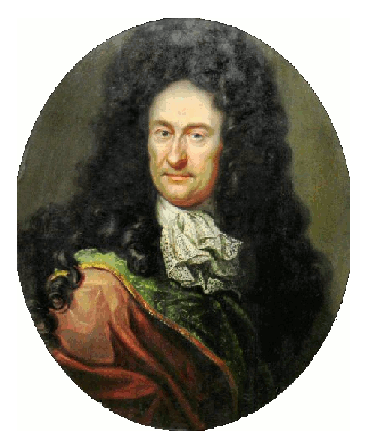
\includegraphics[height=6cm]{Organisation_gestion_donnees/Images/D5_intro_Leibniz}
   \caption{Gottfried Wilhelm Leibniz, 1\,700. © Johann Friedrich Wentzel}
\end{figure}

\begin{prerequis}[Un peu d'histoire]
  L'idée de relation entre des quantités est très ancienne. Le premier âge de l'idée de fonction est celui de l'antiquité avec notamment les mathématiciens babyloniens qui usaient largement des tables sexagésimales de réciproques, de carrés, de racines carrées, de cubes\dots{} Mais peut-on dire que l'idée de fonction était présente ? Ces tables étaient conçues comme des relations entre des ensembles discrets et finis de quantités constantes, bien loin avant que la quantité variable, et la loi de variation soient exhibées comme des objets mathématiques. \\
   Il faudra attendre la fin du 17\up{e} siècle pour que le terme de fonction (du latin {\it fuctio} qui signifie exécution) soit introduit par le mathématicien allemand {\bf Leibniz Gottfried}, dans un cadre géométrique. La notation fx apparaît chez {\bf Léonard Euler} en 1734. \\   
   Actuellement, de multiples fonctions sont représentées dans des tableaux, ou plutôt des tableurs : un logiciel qui permet de manipuler des données numériques, d'effectuer un certain nombre d'opérations de façon automatisée en utilisant des fonctions prédéfinies. \\
   Le premier tableur fut créé en 1978 par {\bf Daniel Bricklin}, étudiant à Harvard qui devait créer des tableaux comptables pour une étude de cas sur Pepsi-Cola sans pour autant établir tous les calculs \og à la main \fg. Son premier prototype, {\it VisiCalc} (pour Visible Calculator), pouvait manipuler un tableau de vingt lignes et cinq colonnes !
\end{prerequis}


\cours %%%%%%%%%%%%%%%%%%%%%%%%%%%%%
%%%%%%%%%%%%%%%%%%%%%%%%%%%%%%%%

\section{Généralités sur les fonctions} %%% 1

\subsection{Définitions} % A

\begin{definition}[Fonction, image, antécédent]
   Une \textbf{fonction} est une relation qui, à chaque élément $x$ d'un ensemble $\mathcal{D}$ appelé ensemble de définition, est associé un unique élément $y$. \\
   On note: $y=f(x)$\quad ou \quad $f:x\mapsto f(x)$ \quad ou encore \quad $x \stackrel{f}{\mapsto} f(x)$. \\
   $y$ est l'\textbf{image} de $x$ par $f$ et $x$ est un \textbf{antécédent} de $y$ par $f$.
\end{definition}

\begin{remarque}
   il y a toujours une image, mais il peut y avoir aucun, un ou plusieurs antécédents.
\end{remarque}

\begin{exemple*1}
   Soit $f$ la fonction définie sur $\R$ par $f(x)=x^2+3$.
   \begin{itemize}
      \item Pour calculer l'image d'un nombre $x$ par $f$, il suffit de remplacer le \og $x$ \fg{} dans l'expression de $f$ : l'image de $5$ par $f$ est $f(5)=5^2+3=28$.
      \item Pour calculer les éventuels antécédents d'un nombre $y$ par $f$, il faut résoudre l'équation $f(x) =y$ :
      \begin{itemize}
         \item[--] les antécédents de 7 vérifient $f(x)=7$ c'est à dire $x^2+3=7 \iff x^2 =4 \iff x=-2$ ou $x=2$ ; il y a deux antécédents de 7 par $f$.
         \item[--] les antécédents éventuels de 1 vérifieraient $f(x)=1$ c'est à dire $x^2+3=1 \iff x^2 =-2$ ; \\
         cette équation est impossible car un carré ne peut pas être négatif, donc il n'y a pas d'antécédent de 1 par $f$.
         \item[--] l'antécédent de $3$ vérifie $f(x)=3$ c'est à dire $x^2+3=3 \iff x^2 =0 \iff x=0$ ; \\
         il y a un seul antécédent de $3$ par $f$.
      \end{itemize}
   \end{itemize}
\end{exemple*1}


\subsection{Différents modes de représentation} % B

On souhaite représenter la fonction $f$ définie sur $\R$ par : $f(x)=x^2-4x+1$.

\begin{minipage}{9cm}   
   On peut trace par exemple la portion de courbe représentative de $f$ dont les abscisses sont comprises entre $-1$ et $5$. \\   
   On commence par compléter un tableau de valeurs :
   \begin{center}  
   \begin{Ctableau}{0.7\linewidth}{8}{c}
      \hline
      $x$ & $-1$ & 0 & 1 & 2 & 3 & 4 & 5 \\
      \hline
      $f(x)$ & 6 & 1 & $-2$ & $-3$ & $-2$ & 1 & 6 \\
      \hline
   \end{Ctableau}
   \end{center}     
   Puis on place les points de coordonnées $M(x,f(x))$ dans le repère ci-contre avant de tracer \og à main levée \fg{} la courbe passant par les points. \\ [5mm]
   {\it la touche 
\includegraphics[width=1cm]{Organisation_gestion_donnees/Images/D5_cours_fx} de la calculatrice TI-Collège Plus permet de créer une table de valeurs.} 
\end{minipage}
\qquad
\begin{minipage}{6cm}
   {\psset{yunit=0.75}
   \begin{pspicture}(-1,-4)(5,6.5)
      \mili{-1}{-4}{5}{6}
      \psaxes{->}(0,0)(-1,-4)(5.2,6.2)
      \psdots[linecolor=B2,linewidth=2pt](-1,6)(0,1)(1,-2)(2,-3)(3,-2)(4,1)(5,6)
      \psplot[linecolor=B2,linewidth=2pt]{-1}{5}{x x mul 4 x mul sub 1 add}
       \rput(4.3,5){$\mathcal{C}_f$}
       \rput(-0.3,-0.3){0}
   \end{pspicture}}
\end{minipage} 
    
\begin{definition}[Courbe]
   Dans un repère (ici cartésien) OIJ, l'ensemble des points $M$ de coordonnées $(x,f(x))$ forme la \textbf{courbe représentative de la fonction $f$}, souvent notée $\mathcal{C}_f$.
\end{definition}

\smallskip

\begin{remarque}
   on attribue au mathématicien et philosophe français {\it René Descartes} l'invention des repères cartésiens : il associe à un point deux nombres, le nombre $x$ mesurant la distance par rapport à une droite et le nombre $y$ mesurant la distance qui s'applique par ordre à cette droite, d'où le nom ordonnée. 
\end{remarque}

\bigskip

\begin{methode*2*2}[Lecture d'une image ou d'un antécédent]
\begin{itemize}
   \item Pour lire l'{\bf image} d'un nombre $x$ par une fonction $f$, on détermine l'ordonnée de la courbe d'abscisse $x$.
   \item Pour lire le ou les {\bf antécédents} de $y$ par une fonction $f$, on détermine le ou les abscisses de la courbe d'ordonnée $y$.
\end{itemize}
\exercice
   Déterminer l'image de 1 par la fonction $f$. \\
   \begin{pspicture}(-1.5,-3.3)(5,3.5)
      \mili{-1}{-3}{5}{3}
      \psaxes{->}(0,0)(-1,-3)(5,3)
      \rput(-0.3,-0.3){0} 
      \psplot[linecolor=B2,linewidth=1.5pt]{-0.4}{4.4}{x x mul 4 x mul sub 1 add}
      \psline[linecolor=A1,linewidth=1.5pt]{->}(1,0)(1,-2)
      \psline[linecolor=A1,linewidth=1.5pt]{->}(1,-2)(0,-2)
      \rput(4,2.5){$\mathcal{C}_f$}
   \end{pspicture}
\correction
   On se place en $x=1$ sur l'axe des abscisses, puis on se déplace verticalement jusqu'à rencontrer $\mathcal{C}_f$. Enfin, on lit $y =f(x)$ sur l'axe des ordonnées : \\
   \bm{l'image de $1$ par $f$ est $-2$}
\exercice
   Déterminer le ou les antécédent(s) de 1 par la fonction $f$. \\
   \begin{pspicture}(-1.5,-3.3)(5,3.5)
      \mili{-1}{-3}{5}{3}
      \psaxes{->}(0,0)(-1,-3)(5,3)
      \rput(-0.3,-0.3){0}
      \psplot[linecolor=B2,linewidth=1.5pt]{-0.4}{4.4}{x x mul 4 x mul sub 1 add}
      \psline[linecolor=A1,linewidth=1.5pt]{-}(-1,1)(5,1)
      \psline[linecolor=A1,linewidth=1.5pt]{->}(0,1)(0,0)
      \psline[linecolor=A1,linewidth=1.5pt]{->}(4,1)(4,0)
      \rput(4,2.5){$\mathcal{C}_f$}
   \end{pspicture}
\correction
   On trace la droite horizontale d'ordonnée $y=1$. À partir des points d'intersection avec la courbe, on se déplace verticalement vers l'axe des abscisses pour lire les antécédents : \\
   \bm{les antécédents de $1$ par $f$ sont $0$ et $4$}
\end{methode*2*2}

\bigskip


\begin{definition}[Maximum, minimum]
On dit que la fonction $f$ admet un \textbf{maximum} $M$ [resp. \textbf{minimum} $m$] sur un intervalle $I$, atteint en $x_0$ si, quel que soit le réel $x$ dans $I$, on a $f(x) \leqslant M$ [resp. $f(x) \geqslant m$].
\end{definition}

\begin{exemple*1}
   La courbe précédente admet $-3$ comme minimum, il est atteint pour $x =2$.
\end{exemple*1}

\smallskip

\begin{exemple*1}
   Albert part faire du ski et décide de dévaler une piste sur laquelle il effectue un saut. La hauteur du saut par rapport au sol de la piste s'exprime en fonction du déplacement horizontal, $x$, par la fonction $S:x\mapsto 2,5-\frac{(2x-55)^2}{1\,210}$ où $x$ et $S(x)$ sont exprimés en mètre.
\begin{enumerate}
   \item Calculer l'image de 10 par la fonction $S$. Interpréter ce résultat.
   \item On a tracé la courbe représentative de cette fonction $S$.
   \begin{center}
   \begin{pspicture}(-1,0.1)(12,3.1)
       \mili{0}{0}{12}{3}
       {\psset{xunit=0.2}
       \footnotesize
       \psaxes[Dx=5,Dy=1]{->}(0,0)(60,3)
       \psplot[algebraic=true,linewidth=1.5pt]{0}{55}{2.5-(2*x-55)^2/1210}}
   \end{pspicture}
   \end{center}
  \begin{enumerate}
      \item Que représente, pour Albert, la valeur 55 sur l'axe des abscisses ?
      \item Déterminer graphiquement quelle a été la hauteur maximale du saut d'Albert.
   \end{enumerate}
   \vspace*{-5mm}
   \item Retrouver, par le calcul, la hauteur maximale du saut d'Albert. \\
\end{enumerate}
\correction
\begin{enumerate}
   \item $S(10) =2,5-\frac{(2\times10-55)^2}{1\,210} \approx 1,49$. Cela signifie que, quand Albert s'est déplacé horizontalement de 10 m, il est à environ 1,49 m du sol.
   \item
   \begin{enumerate}
      \item  55 m est la longueur du saut, mesurée en déplacement horizontal.
      \item La hauteur maximale du saut d'Albert est d'environ 2,5 m, elle correspond à une déplacement horizontal d'environ 27,5 m.
   \end{enumerate}
   \item L'expression $S$ est la somme de deux termes dont le premier est fixe et le second est négatif ou nul puisque $(2x -55)^2$ est un carré, positif ou nul. Il en résulte que la valeur de $S$ est maximale lorsque  $(2x -55)^2$ est nul, donc lorsque $2x =55$ soit $x =\frac{55}{2} =27,5$. \\
   Dans ce cas, $S =2,5$. Donc, la hauteur maximale du saut d'Albert est de 2,5 m. \\ [-10mm]
\end{enumerate}
\end{exemple*1}  


%%%%%%%%%%%%%%%%%%%%%%%
\section{Fonctions affines et linéaires} %%% 2

\begin{definition}[Fonction affine, linéaire]
   Soient $a$ et $b$ deux réels donnés. La fonction définie sur $\R$ par $f(x)=ax+b$ est appelée \textbf{fonction affine}, elle est représentée par une droite où
   \begin{itemize}
      \item le réel $a$ est le coefficient directeur de cette droite ;
      \item le réel $b$ est l'ordonnée à l'origine.
   \end{itemize}
   Si $b=0$, il s'agit d'une \textbf{fonction linéaire} représentée par une droite passant par l'origine.
\end{definition}

\smallskip

Comme pour n'importe quelle fonction, pour tracer une fonction affine, on choisit des points que l'on place dans un repère (deux suffisent). Dans le cas d'une fonction linéaire, il suffit d'un point en plus de l'origine.

\begin{exemple}[0.3]
   $\mathcal{C}_1:f(x)=x+1$ \\
   $\mathcal{C}_2:f(x)=2$ \\
   $\mathcal{C}_3:f(x)=-3x$ \\
   $\mathcal{C}_4:f(x)=\frac34x-3$.
\correction
   {\psset{unit=0.3}
   \begin{pspicture}(-11,-4)(18,3)
         \psgrid[subgriddiv=1,griddots=10,gridlabels=0,gridcolor=lightgray](-4,-4)(4,4)
      \small
      \psaxes[labels=none]{->}(0,0)(-4.5,-4.5)(4.5,4.5)
      \rput(1,-0.3){$1$}
      \rput(-0.3,1){$1$}
      \psline[linewidth=0.1,linecolor=B2](-4,2)(4,2)
      \rput(-3.3,2.4){\textcolor{B2}{$\mathcal{C}_2$}}
      \psline[linewidth=0.1,linecolor=A1](-4,-3)(3,4)
      \rput(-3,-1.5){\textcolor{A1}{$\mathcal{C}_1$}}
      \psline[linewidth=0.1,linecolor=G1](-1.33,4)(1.33,-4)
      \rput(1.8,-3.6){\textcolor{G1}{$\mathcal{C}_3$}}
      \psline[linewidth=0.1,linecolor=J1](-1.33,-4)(4,0)
      \rput(3,-1.4){\textcolor{J1}{$\mathcal{C}_4$}}
      \rput(12,0){\parbox{3.3cm}{La fonction est croissante si $a$ est positif, constante si $a$ est nul et décroissante si $a$ est négatif.}}
   \end{pspicture}}
\end{exemple}


%%%%%%%%%%%%%%%
\section{Tableurs} %%%%% 3

   Un tableur est un logiciel d'édition et de présentation de tableaux. Il comporte des \textbf{feuilles de calcul} composées de multiples lignes et colonnes formant des \textbf{cellules}. Chaque cellule est repérée par son adresse : une lettre désignant la colonne et un numéro désignant la ligne. Par exemple, la cellule A1 fait référence à la colonne A ligne numéro 1.

\begin{remarques}
   \begin{itemize}
      \item La taille d'une cellule est variable, ses dimensions peuvent être modifiées.
      \item La virgule pour noter les nombres décimaux se traduit par un point dans certains logiciels.
      \item Une cellule peut contenir trois types de données : du texte, un nombre ou une formule.
   \end{itemize}
\end{remarques}


\subsection{Saisie d'une formule dans une cellule} %%% A

\begin{propriete}[Syntaxe d'une formule]
   Pour saisir une formule dans une cellule, il faut commencer par le signe {\blue $=$} pour indiquer qu'il s'agit d'un calcul.
\end{propriete}
  
\begin{remarque}
    si on oublie le signe \cell{\texttt{=}} le contenu de la cellule n'est pas interprété comme une formule : 
    \begin{itemize}
       \item l'écriture de \Cell{\texttt{1+2}} donne\,\Cell{\texttt{1+2}}
       \item l'écriture de \Cell{\texttt{=1+2}} donne\,\Cell{\texttt{3}}
    \end{itemize}
\end{remarque}   

\bigskip

{\renewcommand{\StringDOCUMENTATION}{Exemples d'éléments}
\begin{documentation}
   \begin{itemize}
      \item Coordonnées de cellule, par exemple \Cell{\texttt{=C5}}
      \item Opérateurs de calcul : addition \cell{\texttt{+}} soustraction \cell{\texttt{-}} multiplication \cell{\texttt{*}} division \cell{\texttt{/}}
      \item Fonctions : \Cell{\texttt{=SOMME()}} \Cell{\texttt{=MOYENNE()}} \\ [-6mm]
   \end{itemize}
\end{documentation}}

\begin{exemple*1}
   on souhaite calculer la moyenne arithmétique de quatre notes à l'aide d'un tableur :
   \begin{center}
   \textsf{
      \begin{tabular}{|>{\columncolor{lightgray!30}}c|p{1.5cm}|C{1.5}|p{3.5cm}|p{3.5cm}|}
         \hline
         \rowcolor{lightgray!30} & \centering A & B & \centering C & \centering D \tabularnewline
         \hline
         1 & Note 1 & 12 & Moyenne méthode 1 & \texttt{=(B1+B2+B3+B4)/4} \\
         \hline
         2 & Note 2 & 15 & Moyenne méthode 2 & \texttt{=SOMME(B1:B4)/4} \\
         \hline
         3 & Note 3 & 10 & Moyenne méthode 3 & \texttt{=MOYENNE(B1:B4)} \\
         \hline
         4 & Note 4 & 13 & & \\
         \hline
      \end{tabular}}
   \end{center}
   On peut utiliser (au minimum) trois méthodes :
   \begin{itemize}
       \item la première reprend la définition de la moyenne comme la somme des notes B1+ B2 + B3 + B4 divisée par le nombre total de notes ;
       \item la seconde est équivalente, mais utilise la fonction SOMME() du tableur pour calculer directement la somme de B1 à B4 ;
       \item la troisième utilise directement le fonction MOYENNE() du tableur. \\ [-8mm]
    \end{itemize}
\end{exemple*1}

\bigskip

   L'avantage d'un tableur réside dans le fait que le résultat de la formule est dynamique : il dépend du contenu des cellules mentionnées (B1 à B4 dans l'exemple). Chaque fois que ce contenu est modifié, le tableur recalcule automatiquement le résultat de la formule sans aucune intervention de l'utilisateur.


\subsection{Copie de cellules et adressages} %%%B

   Pour recopier le contenu d'une cellule vers d'autres cellules, on peut utiliser les fonctions \og copier-coller \fg{} ou \og tirer le contenu aux cellules continues \fg{} (sélectionner la croix en bas à droite de la cellule et étendre aux cellules voulues).
   
\begin{propriete}[Adressage relatif]
   Lorsque l'on copie la formule de calcul d'une cellule et qu'on la colle dans une autre cellule, le tableur change automatiquement les numéros de colonnes et de lignes des cellules intervenant dans la formule. Il s'agit d'un \textbf{adressage relatif}. 
\end{propriete}

\begin{exemple*1}
   Maria revient de la boulangerie avec 8 petits gâteaux qu'elle a payés 11,50 \euro{} au total. Il y a des macatias à 0,80 \euro{} l'un et des tartelettes à 2,50 \euro{} pièce. \\
   On veut connaître le nombre de macatias et de tartelettes ramenées en utilisant un tableur.
   \correction
      On commence par indiquer dans la \textbf{ligne 1} les données, ce sont des données de type \og texte \fg{}, puis, on effectue une simulation de tous les cas possibles : on commence par exemple par le cas où il y a 0 macatia et on complète la \textbf{ligne 2} : 
      \begin{center}
      \textsf{
         \begin{tabular}{|>{\columncolor{lightgray!30}}c|C{1.5}|C{1.5}|C{1.5}|C{1.5}|C{1.5}|}
            \hline
            \rowcolor{lightgray!30} & A & B & C & D & E \\
            \hline
            1 & \cellcolor{FondTableaux}{Nombre de macatias} & \cellcolor{FondTableaux}{Nombre de tartelettes} & \cellcolor{FondTableaux}{Prix des macatias} & \cellcolor{FondTableaux}{Prix des tartelettes} & \cellcolor{FondTableaux}{Prix payé} \\
            \hline
            2 & 0 & \texttt{=8-A2} & \texttt{=A2*0,8} & \texttt{=B2*2,5} & \texttt{=C2+D2} \\
            \hline
         \end{tabular}}
      \end{center}
      \begin{itemize}
         \item \textbf{B2 :} le nombre total de gâteaux est 8, pour connaître le nombre de tartelettes, on effectue l'opération \og 8 - nombre de macatias \fg{}, qui est fourni pas la cellule A2 ;
         \item \textbf{C2 :} le prix d'un macatia est de 0,80 \euro, qu'il faut multiplier par le nombre de macatias ;
         \item \textbf{D2 :} le prix d'une tartelette est de 2,50 \euro, qu'il faut multiplier par le nombre de tartelettes fourni pas la cellule B2 ;
         \item \textbf{E2 :} le prix total se calcule par somme du prix des macatias (C2) et des tartelettes (D2).
      \end{itemize}  
      Il suffit ensuite de recopier cette ligne 2 vers le bas jusqu'à 8 macatias en ayant pris soin au préalable de remplir la \textbf{colonne A} comportant le nombre de macatias de 0 à 8. On obtient :
      \begin{center}
      \textsf{
         \begin{tabular}{|>{\columncolor{lightgray!30}}c|C{1.5}|C{1.5}|C{1.5}|C{1.5}|C{1.5}|}
            \hline
            \rowcolor{lightgray!30} & A & B & C & D & E \\
            \hline
            1 & \cellcolor{FondTableaux}{Nombre de macatias} & \cellcolor{FondTableaux}{Nombre de tartelettes} & \cellcolor{FondTableaux}{Prix des macatias} & \cellcolor{FondTableaux}{Prix des tartelettes} & \cellcolor{FondTableaux}{Prix payé} \\
            \hline
            2 & 0 & 8 & 0 & 20 & 20 \\
            \hline
            3 & 1 & 7 & 0,8 & 17,5 & 18,3 \\
            \hline
            4 & 2 & 6 & 1,6 & 15 & 16,6 \\
            \hline
            5 & 3 & 5 & 2,4 & 12,5 & 14,9 \\
            \hline
            6 & 4 & 4 & 3,2 & 10 & 13,2 \\
            \hline
            \rowcolor{B3} 7 & {\bf 5} & {\bf 3} & 4 & 7,5 & {\bf 11,5} \\
            \hline
            8 & 6 & 2 & 4,8 & 5 & 9,8 \\
            \hline
            9 & 7 & 1 & 5,6 & 2,5 & 8,1 \\
            \hline
            10 & 8 & 0 & 6,4 & 0 & 6,4 \\
            \hline
         \end{tabular}}
      \end{center}
      Le prix payé est obtenu dans la cellule E7. Il correspond à l'achat de 5 macatias et de 3 tartelettes. 
\end{exemple*1}

   Au contraire, on souhaite parfois introduire dans une formule les références d'une cellule de telle sorte que cette référence ne change pas lorsque l'on copiera la formule dans une autre cellule.
   
\begin{propriete}[Adressage absolu]
   Dans le cas où la copie ne doit pas modifier la référence, on ajoute le symbole \$ devant le numéro de ligne ou de colonne que l'on souhaite fixer dans la copie de la cellule. Il s'agit alors d'un \textbf{adressage absolu}.
\end{propriete}

\begin{exemple}[0.5]
   On souhaite construire la table de multiplication de 1 à 5. Pour cela, on va utiliser le tableur avec comme données initiales dans la \textbf{ligne 1} et la \textbf{colonne A} les nombres de 1 à 5.
   \begin{center}
   \textsf{
   {\hautab{1}
      \begin{tabular}{|>{\columncolor{lightgray!30}}C{0.4}|C{0.4}|C{0.4}|C{0.4}|C{0.4}|C{0.4}|C{0.4}|}
         \hline
         \rowcolor{lightgray!30} & A & B & C & D & E & F \\
         \hline
         1 & \cellcolor{B3}{$\times$} & \cellcolor{FondTableaux}{1} & \cellcolor{FondTableaux}{2} & \cellcolor{FondTableaux}{3} & \cellcolor{FondTableaux}{4} & \cellcolor{FondTableaux}{5} \\
         \hline
         2 & \cellcolor{FondTableaux}{1} & 1 & 2 & 3 & 4 & 5 \\
         \hline
         3 & \cellcolor{FondTableaux}{2} & 2 & 4 & 6 & 8 & 10 \\
         \hline
         4 & \cellcolor{FondTableaux}{3} & 3 & 6 & 9 & 12 & 15 \\
         \hline
         5 & \cellcolor{FondTableaux}{4} & 4 & 8 & 12 & 16 & 20 \\
         \hline
         6 & \cellcolor{FondTableaux}{5} & 5 & 10 & 15 & 20 & 25 \\
         \hline
      \end{tabular}}}
   \end{center}
   \correction
      On peut procéder par étapes :
      \begin{itemize}
         \item dans la cellule B2, on écrit \Cell{\texttt{=B1*A2}}
         \item en recopiant vers la droite, la cellule A2 doit rester fixe, donc la colonne A ne doit pas être modifiée. On écrit alors \Cell{\texttt{=B1*\$A2}}
         \item en recopiant vers le bas, la cellule B1 doit rester fixe, donc la ligne 1 ne doit pas être modifiée. On écrit alors \Cell{\texttt{=B\$1*\$A2}} \\
      \end{itemize}
      Cette dernière formule étant valable pour toutes les cellules, il suffit de la recopier jusqu'à F6. 
\end{exemple}



%%%%%%%%%%%%%%%%%%%%%%%%%%%%%%%
%%%%%%%%%%%%%%%%%%%%%%%%%%%%%%%
\activites

\begin{activite}[Groupement 1 - Exercice 1 - Partie 2 - Question 2 : tableur]
   \ \\ [-16mm]
   \begin{QCM}
      Dans une version adaptée du biathlon, les élèves ont à parcourir, en courant, 4 grands tours tracés avec des plots sur un stade. À l'issue de chacun des 3 premiers tours, ils se présentent au pas de tir et lancent trois balles sur des cibles. S'ils atteignent 3 fois leur cible, ils n'ont pas de pénalité et repartent pour le grand tour suivant. En revanche, pour chaque lancer manqué, ils doivent effectuer un petit tour avant de repartir sur le grand tour. \\
      Pour chaque élève on mesure la durée mise pour faire un parcours complet (grands tours + lancers + petits tours de pénalité le cas échéant). L'objectif est de mettre le moins de temps possible pour effectuer le parcours complet.
      Le professeur des écoles souhaite aider ses élèves à développer une stratégie pour améliorer leurs résultats. Il relève les performances d’un même élève de {\small CE1} qui fait 3 fois l’épreuve de biathlon dans sa totalité en modifiant certains paramètres à chaque essai. Dans le tableau, $V_{\text{moy}}$ est la vitesse moyenne de cet élève sur les périodes de course (4 grands tours + éventuels tours de pénalités).
      \begin{enumerate}
         \item La formule saisie en \texttt{H3} puis recopiée vers le bas est \texttt{=1000+(C3+E3+G3)*20}. \\
            Expliquer le terme \texttt{(C3+E3+G3)*20} dans le contexte de l’exercice.          
         \item Donner une formule qui a pu être introduite dans la cellule \texttt{J3}, de telle sorte qu’elle a pu être recopiée vers le bas pour effectuer le calcul pour les autres essais.               
         \item Donner une formule qui a pu être introduite dans la case \og durée totale \fg{} \texttt{K3}, de telle sorte qu’elle a pu être recopiée vers le bas pour effectuer le calcul pour les autres essais.         
         \item Interpréter le tableau pour déterminer ce que l’élève a modifié entre l’essai 2 et l’essai 3.         
         \item Si on analyse les performances de l’élève aux essais 2 et 3, quelle hypothèse ce tableau permet-il de faire du point de vue des stratégies à adopter ?
      \end{enumerate}
         \begin{center}
         {\hautab{1.2}{\scriptsize\texttt{
         \begin{tabular}{|>{\columncolor{lightgray}}C{0.3}|*{11}{C{0.92}|}}
            \hline
            \rowcolor{lightgray} & A & B & C & D & E & F & G & H & I & J & K \\
            \hline
            1 & \multirow{3}{*}{élève} & \multicolumn{2}{c|}{tirs n°1} & \multicolumn{2}{c|}{tirs n°2} & \multicolumn{2}{c|}{tirs n°3} & distance & temps & $V_{\text{moy}}$ & durée \\
           \cline{1-1} \cline{3-8}
           & & durée & cibles & durée & cibles & durée & cibles & totale & course & (m/min) & totale \\
            2 & & (s) & manquées & (s) & manquées & (s) & manquées & parcourue & (s) & & (min) \\
            \hline
            3 & essai 1 & 30 & 0 & 30 & 1 & 30 & 2 & 1060 & 482 & 132 & 9,53 \\
            \hline
            4 & essai 2 & 30 & 0 & 32 & 0 & 35 & 0 & 1000 & 469 & 128 & 9,43\\
            \hline
            5 & essai 3 & 19 & 3 & 21 & 3 & 21 & 3 & 1180 & 566 & 125 & 10,45 \\
            \hline
         \end{tabular}}}} \medskip
      \end{center}
   \end{QCM}
   
   \bigskip
   
   \textcolor{G1}{
   {\bf Exemple de corrigé.} \smallskip
      \begin{enumerate}
         \item \texttt{(C3+E3+G3)} correspond à la somme des tirs ratés. Chaque tir raté ayant comme effet de faire un tour de pénalité de 20 m, la formule \texttt{(C3+E3+G3)*20} correspond à \uline{la distance supplémentaire parcourue en raison des cibles loupées}, exprimée en mètre.
         \item La vitesse moyenne se calcule en divisant la distance totale parcoure (donnée par la colonne \texttt{H} et exprimée en mètre) par le temps de course (donné par la colonne \texttt{I} et exprimé en seconde). \\
               Pour obtenir la vitesse moyenne en m/min, il faut convertir la durée en minute, donc la diviser par 60. \\
               \uline{Une formule introduite en \texttt{J3} peut alors être : \texttt{=H3/(I3/60)}.}
         \item La durée totale, en minute, est la somme du temps de course et du temps passé sur pour chacun des trois tirs. Ceux-ci étant exprimés en seconde, il faut diviser le tout par 60 pour obtenir des minutes. \\
            On peut, par exemple, introduire \uline{la formule \texttt{=(B3+D3+F3+I3)/60} dans la case \texttt{K3}} avant de l'étirer vers le bas.
         \item \uline{Entre l'essai 2 et l'essai 3, l'élève a décidé de tirer plus vite}.
         \item En observant la durée total aux essais 2 et 3, on constate que l'élève a mis une minute de moins au total alors qu'il a passé plus de temps sur le pas de tirs (essai 2), puisqu'il a dû parcourir plus de distance. On peut donc dire que, dans ce cas, \uline{la stratégie à adopter serait de prendre son temps à bien viser et  commettre moins de faute au lieu de se précipiter pour terminer son tir plus rapidement et devoir effectuer des tours de pénalité}.
      \end{enumerate}}
\end{activite}

\pagebreak


\begin{activite}[Groupement 1 - Exercice 5 - Questions 5 à 7 : fonction affine et tableur]
   \ \\ [-16mm]
   \begin{QCM}
      Un ballon-sonde est un ballon à gaz utilisé pour faire des mesures locales dans l'atmosphère. \\
   Dans le cadre du projet scientifique qu’elle anime pour sa classe de CM2, une professeure des écoles a reçu un petit ballon-sonde. Son enveloppe, composée de matières plastiques et de latex, a la forme, une fois gonflée, d'un cône de révolution surmonté d'une demi-sphère. \\ 
   La pression atmosphérique diminuant avec l'altitude, le ballon se dilate en prenant de la hauteur et ses dimensions augmentent jusqu’à l’éclatement après une ascension de plus de vingt kilomètres.
   \begin{enumerate}
      \item On lâche le ballon à 0 mètre d’altitude. On relève alors une température de 15°C. \\
         À 4 500 mètres d'altitude, la température transmise est de $-$12°C. Entre 0 et 12 000 m d’altitude, la température, en degré Celsius, en fonction de l’altitude $x$, en mètre, peut être modélisée par une fonction affine notée $t$. \\
         Montrer que pour tout $x$ entre 0 et 12 000, on a $t(x) = -0,006x + 15$.            
      \item À partir de quelle altitude la température devient-elle négative ? \\
         Justifier le résultat en résolvant une inéquation.    
      \item La professeure des écoles a réalisé, à l’aide d’un tableur, le calcul des températures en fonction de l’altitude du ballon-sonde. \medskip
      \begin{center}
         {\hautab{1.3}{\footnotesize\texttt{
         \begin{tabular}{|>{\columncolor{lightgray}}C{0.1}|C{1.5}|*{13}{C{0.55}|}}
            \hline
            \rowcolor{lightgray} & A & B & C & D & E & F & G & H & I & J & K & L & M & N \\
            \hline
            1 & altitude en mètre & 0 & 500 & 1000 & 1500 & 2000 & 2500 & 3000 & 3500 & 4000 & 4500 & 5000 & 5500 & 6000 \\
            \hline
            2 & température en degré & 15 & 12 & 9 & 6 & 3 & 0 & $-3$ & $-6$ & $-9$ & $-12$ & $-15$ & $-18$ & $-21$  \\
            \hline
            \hline
            1 & altitude en mètre & 6500 & 7000 & 7500 & 8000 & 8500 & 9000 & 9500 & 10000 & 10500 & 11000 & 11500 & 12000 & \\
            \hline
            2 & température en degré & $-24$ & $-27$ & $-30$ & $-33$ & $-36$ & $-39$ & $-42$ & $-45$ & $-48$ & $-51$ & $-54$ & $-57$ & \\
            \hline
         \end{tabular}}}}
      \end{center}
      \medskip
      En observant les données du tableau, sachant que le ballon part de 0 mètre d'altitude, à quelle altitude se trouve-t-il lorsque la température a baissé de 30°C? \\
   \end{enumerate}
   \end{QCM}
   
   \bigskip
   
   \textcolor{G1}{
   {\bf Exemple de corrigé.} \smallskip
      \begin{enumerate}
         \item On considère la fonction affine d'équation $t(x) =ax+b$. \\
            À 0 mètre d’altitude, la température est de 15°C donc : $t(0) =a\times0+b =15 \iff b =15$. \\
            À 4 500 mètres d’altitude, la température est de $-12$°C donc : $t(4\,500) =a\times(4\,500)+15 =-12$ \\
            Soit, $4\,500\,a =-12-15 =-27$ \\
            $\iff a =-27\div4\,500 = -0,006$. \\
            \uline{Pour tout $x$ entre 0 et 12 000, $t(x) =-0,006x+15$.}
            \item La température devient négative lorsque $t(x)<0$, soit $-0,006x+15<0$ \\
            \hspace*{7.1cm} $\iff -0,006x<-15$ \\ [1mm]
            \hspace*{7.1cm} $\iff x>\dfrac{-15}{-0,006}$ \\ [1mm]
            \hspace*{7.1cm} $\iff x>2\,500$. \\
            \uline{La température devient négative à partir de 2 500 mètres d'altitude}.
         \item La température aura baissé de 30°C lorsque celle-ci sera de $-15$°C. \\
            Dans le tableau, on peu lire que \uline{cette température est atteinte à 5 000 mètres d'altitude}.
      \end{enumerate}}
\end{activite}

\pagebreak


\begin{activite}[Groupement 2 - Exercice 3 - Partie B - Question 5 : lecture, inéquation]
   \ \\ [-16mm]
   \begin{QCM}
      On considère les fonctions $f$ et $g$ définies pour tout $x$ compris entre 0 et 5 par :
      $$f(x) =210-14x \quad \text{et} \quad g(x) =112x$$
      $f$ représente le volume d'un socle en bois d'un trophée, sur lequel on pose une pyramide en verre de volume $g$. \\
      On a représenté dans un repère orthogonal ces deux fonctions.
       \begin{center}
      {\psset{yunit=1.2}
         \begin{pspicture}(-0.5,-0.3)(10.4,6.2)
            \psgrid[subgriddiv=5, gridlabels=0pt,subgridcolor=lightgray,](0,0)(10,6)
            \psaxes[dx=1,Dx=0.5,dy=1,Dy=100]{->}(0,0)(10.4,6.2)
            \psline[linewidth=0.5mm](0,0)(10,5.6)
            \psline[linewidth=0.5mm](0,2.1)(10,1.4)
            \rput(9.7,1.6){$D_1$}
            \rput(9.3,5.5){$D_2$}
         \end{pspicture}}
      \end{center}
      \begin{enumerate}
         \item Déterminer quelle fonction ($f$ ou $g$) est représentée par chacune des droites $D_1$ et $D_2$ ? Justifier.
         \item Déterminer avec la précision permise par le graphique les valeurs de $x$ pour lesquelles le volume du socle en bois est inférieur ou égal au volume de la pyramide en verre.
         \item Retrouver le résultat précédent en posant puis en résolvant une inéquation.
      \end{enumerate}
   \end{QCM}
   
   \bigskip
   
   \textcolor{G1}{
   {\bf Exemple de corrigé.} \smallskip
      \begin{enumerate}
         \item $g$ est une fonction linéaire, elle passe par l'origine du repère, c'est donc la droite $D_2$. \\
            $f$ est donc représentées par la droite $D_1$. \\
            \uline{$f$ est représentée par la droite $D_1$ et $g$ par $D_2$}.
         \item Graphiquement, il suffit de déterminer les abscisses pour lesquelles la droite $D_1$ est en dessous de la droite $D_2$. \\
            \uline{Le volume du socle en bois est inférieur ou égal au volume de la pyramide en verre pour des valeurs $x$ supérieures ou égales à 1,65 environ (et inférieures ou égales à 5)}.
         \item On résout l'inéquation : $210-14x \leq 112x \iff 210 \leq 112x+14x$ \\
            \hspace*{6.1cm} $\iff 210 \leq 126x$ \\ [1mm]
            \hspace*{6.1cm} $\iff \dfrac{210}{126} \leq x$ \\ [1mm]
            \hspace*{6.1cm} $\iff \dfrac53 \leq x$. \\ [1mm]
            \uline{Le volume du socle en bois est inférieur ou égal au volume de la pyramide en verre pour des valeurs $x$ comprises entre} $\uline{\dfrac53}$ \uline{et 5 inclus}.
      \end{enumerate}}
\end{activite}

\pagebreak


\begin{activite}[Groupement 2 - Exercice 4 - Question 5 : tableur]
   \ \\ [-16mm]
   \begin{QCM}
      Adam a réalisé un programme à l’aide du logiciel Scratch : soit $x$ le nombre de départ, son programme retourne le nombre $2x^2-x-6$. \\
      Adam souhaite automatiser les calculs de son programme pour les entiers naturels. Il utilise un tableur dont la copie d’écran est donnée ci-dessous. \\
      Quelle formule doit-il saisir dans la case \texttt{B2} pour qu'il puisse l’étirer vers le bas sur l'ensemble de la colonne ?
       \begin{center}
         {\hautab{0.9}\texttt{\small
         \begin{tabular}{|>{\columncolor{lightgray}}C{0.5}|C{3.5}|C{4.5}|}
            \hline
            \rowcolor{lightgray} & A & B \\
            \hline
            1 & Nombre de départ & Résultat du programme \\
            \hline
            2 & 1 & -5 \\
            \hline
            3 & 2 & 0 \\
            \hline
            4 & 3 & 9 \\
            \hline
            5 & 4 & 22 \\
            \hline
            6 & 5 & 39 \\
            \hline
         \end{tabular}}}
      \end{center} \medskip
   \end{QCM}
   
   \bigskip
   
   \textcolor{G1}{
   {\bf Exemple de corrigé.} \\
      \uline{En \texttt{B2}, on peut entrer, par exemple, la formule \texttt{=2*A2*A2-A2-6}.}} \\
\end{activite}

\bigskip


\begin{activite}[Groupement 3 - Exercice 3 - Partie A - Question 4 : lecture graphique]
   \ \\ [-16mm]
   \begin{QCM}
      Le graphique ci-dessous représente l’aire, exprimée en mètre carré, d'un potager $ADEF$ de forme rectangulaire en fonction de la longueur $AD$ en mètre.
      \begin{center}
         \psset{unit=0.35,algebraic=true}
         \small
         \begin{pspicture}(-5,-1)(31,14.5)
            \psgrid[subgriddiv=0,gridlabels=0pt,gridcolor=gray!60](0,0)(31,15)
            \psaxes[dy=1,Dy=5,labelFontSize=\scriptstyle]{->}(31,15)
            \psplot{0}{24}{2*x-x*x/12}
            \rput(27,-2){Longueur $AD$ en m}
            \rput(-6,13.5){Aire de}
            \rput(-5,12.5){$ADEF$ en m$^2$}
         \end{pspicture}
      \end{center}
      À l’aide du graphique, répondre aux questions suivantes :
      \begin{enumerate}
         \item Quelle est l’aire du potager si la longueur $AD$ vaut 5 m ?
          \item Pour quelle(s) valeur(s) de la longueur $AD$ l’aire du potager est-elle égale à 45 m$^2$ ?
          \item Pour quelle(s) valeur(s) de la longueur $AD$ l’aire du potager est-elle supérieure ou égale à 50 m$^2$ ?  
         \item Quelle est l’aire maximale du potager ? Donner la longueur et la largeur du rectangle $ADEF$ correspondant. \medskip
      \end{enumerate}
   \end{QCM}
   
   \bigskip
   
   \textcolor{G1}{
   {\bf Exemple de corrigé.} \smallskip
      \begin{enumerate}
         \item Si $AD =5$ m, alors \uline{l'aire du potager vaut environ 40 m$^2$}.      
         \item L'aire du potager est égale à 45 m$^2$ lorsque \uline{$AD =6$ m ou $AD =18$ m}.
         \item L'aire du potager est supérieure ou égale à 50 m$^2$ lorsque \uline{$AD$ est comprise en 7 m et 17 m environ}.          
         \item L'aire maximale du potager est de \uline{60 m$^2$, atteinte lorsque $AD$ vaut 12 m, et $DE$ vaut alors 5 m}.
      \end{enumerate}}
\end{activite}


%%%%%%%%%%%%%%%%%%%%%%%%%%%%%%%
%%%%%%%%%%%%%%%%%%%%%%%%%%%%%%%
\exercicesbase

\begin{center}
   {\cursive Maîtriser les bases avec} \href{http://mathenpoche.sesamath.net}{
\includegraphics[width=3cm]{Nombres_et_calculs/Images/mathenpoche}} \\
   \bigskip
   {\hautab{0.85}
   \cursive
   \begin{Ltableau}{0.775\linewidth}{4}{C{1}|C{1}|p{7cm}|p{2.3cm}}
      \hline
      Classe & \texttt{N\degre} & Thème & Dans le cours \\
      \hline
      \textcolor{orange}{\bf 6\up{e}} & \texttt{U1} & Utiliser un tableur & 3. \\
      \hline
      \textcolor{violet}{\bf 4\up{e}} & \texttt{B3} & Fonctions & 1. \\
      & \texttt{U1} & Utiliser un tableur & 3. \\
      \hline
      \textcolor{teal}{\bf 3\up{e}} & \texttt{B3} & Fonctions & 1. et 2. \\
      & \texttt{U1} & Utiliser un tableur & 3. \\
      \hline
      \textcolor{red}{\bf 2\up{nde}} & \texttt{F8} & Généralités sur les fonctions & 1. et 2. \\
      & \texttt{U1} & Utiliser un tableur & 3. \\
      \hline
   \end{Ltableau}}
\end{center}

\bigskip


\begin{exercice}[CRPE 2014 G1] %%% 4
   Pour s'entraîner, un cycliste effectue un parcours aller-retour entre deux villes A et B distantes de \ukm{45}.
   \begin{itemize}
      \item Il part de la ville A à 9 h 30 et on considère qu'à l'aller, il roule à une vitesse constante de 30 km/h.
      \item Après un repos d'une heure, il repart de la ville B et cette fois-ci rejoint la ville A à la vitesse constante de 50 km/h.
   \end{itemize} \vspace*{-5mm}
   \begin{enumerate}
      \item À quelle heure arrive-t-il à la ville B ?
      \item Représenter graphiquement la distance entre le cycliste et la ville A sur l'intégralité du parcours. On placera en abscisse l'heure de la journée et en ordonnée la distance entre le cycliste et la ville A exprimée en km.
      \item À quelle heure est-il de retour à la ville A ? Donner le résultat en heures et minutes.
   \end{enumerate}
\end{exercice}

\begin{corrige}
\ \\ [-5mm]
   \begin{enumerate}
      \item Le cycliste parcourt en moyenne \ukm{30} en une heure. Donc, il parcourra \ukm{45} en une heure et trente minutes. {\blue Le cycliste arrivera à 11 heures dans la ville B.}
      \item Représentation graphique du parcours.
         {\psset{xunit=3.5cm,yunit=0.14cm,labelFontSize=\scriptstyle}
         \begin{pspicture}(9,-5)(13,53)
            \psaxes[Ox=9.5,Dx=0.5,Dy=5,xsubticks=2,ysubticks=5,comma]{->}(9.5,0)(13.2,48)
            \pcline(9.5,0)(11,45) \Aput{aller}
            \pcline(11,45)(12,45) \Bput{repos}
            \pcline(12,45)(12.9,0) \Aput{retour}
            \psline[linestyle=dotted](9.5,45)(11,45)
            \psline[linestyle=dotted](11,0)(11,45)
            \psline[linestyle=dotted](12,0)(12,45)
            \rput(13.35,0){\scriptsize heure}
            \rput(9.5,50){\scriptsize distance de A}
         \end{pspicture}}
      \item Il est 12 heures lorsque le cycliste repart (11h + 1h). Sa vitesse est de 50 km/h et il lui faut parcourir 45 km. \\ [1mm]
         D'après la formule $v =\dfrac{d}{t}$, on a $t =\dfrac{d}{v} =\dfrac{\ukm{45}}{50\text{ km/h}} =0,9$ h. \\ [1mm]
         Or, $0,9\times60 =54$, donc le cycliste va mettre 54 minutes pour rentrer. \\
         {\blue Le cycliste sera de retour à la ville A à 12 heures et 54 minutes.} \\
   \end{enumerate}
\end{corrige}

\bigskip


\begin{exercice}[CRPE 2018 G1] %%% 3
   La distance d’arrêt $d_\text{A}$ correspond à la distance de réaction $d_\text{R}$ additionnée à la distance de freinage $d_\text{F}$.
   \begin{center}
      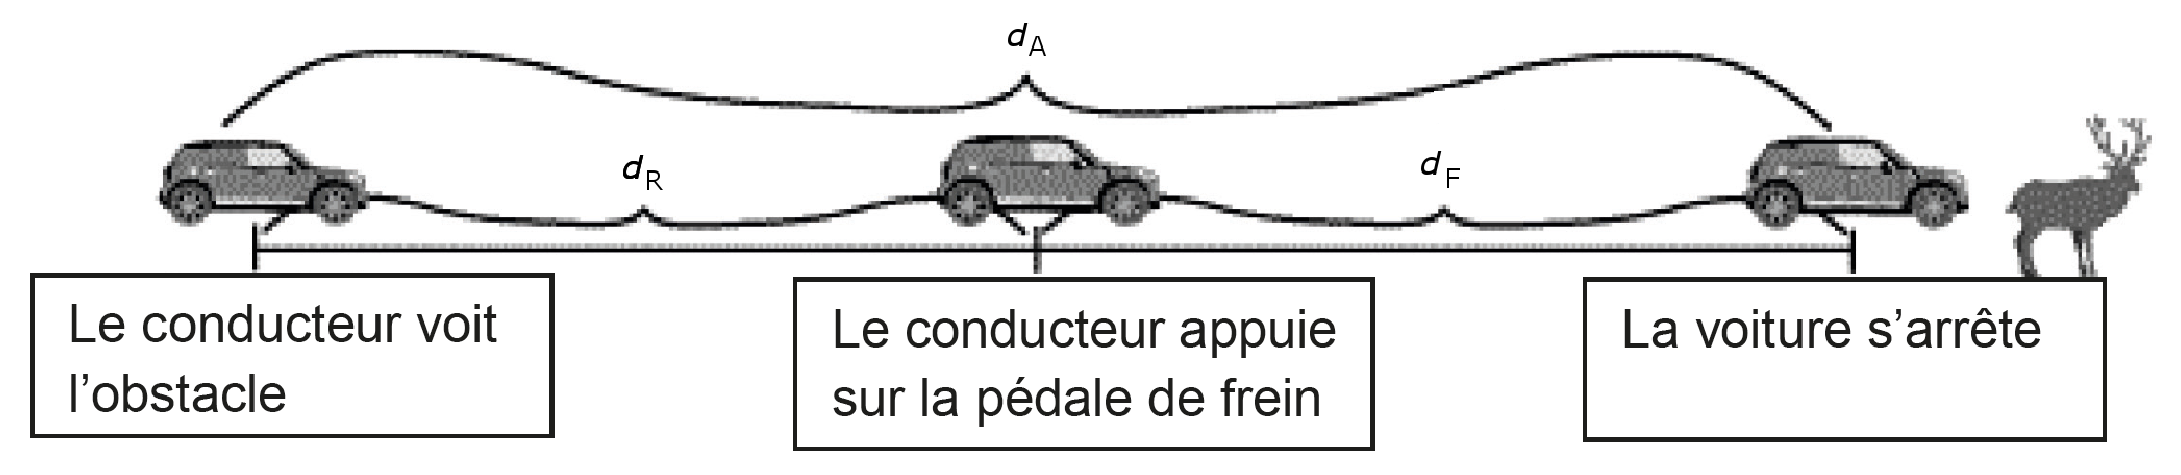
\includegraphics[width=14cm]{Organisation_gestion_donnees/Images/D5_ex_distance_arret}
   \end{center}
   Si $v$ est la vitesse de la voiture au moment où le conducteur voit l’obstacle (en m/s : mètre par seconde), la distance de freinage (en mètre) se calcule de la manière suivante : $d_\text{F} =v^2\times k$ où $k$ est une constante qui dépend de l’état de la route ($k =0,14$ sur route mouillée, et $k =0,073$ sur route sèche). \\
   On admet alors que $$d_\text{A} =v\times t_\text{R}+k\times v^2$$ où $t_\text{R}$ est le temps de réaction, en seconde.
   \begin{enumerate}
      \item On estime qu’un conducteur vigilant a un temps de réaction de 0,75 seconde. Calculer la distance d’arrêt pour un véhicule roulant à 90 km/h sur route mouillée.
      \item Pour un conducteur vigilant, la distance d’arrêt sur route sèche est-elle proportionnelle à la vitesse ? \medskip
      \item Le diagramme ci-dessous représente la distance d’arrêt sur route sèche d’un véhicule en fonction de sa vitesse. \smallskip
         \begin{center}
            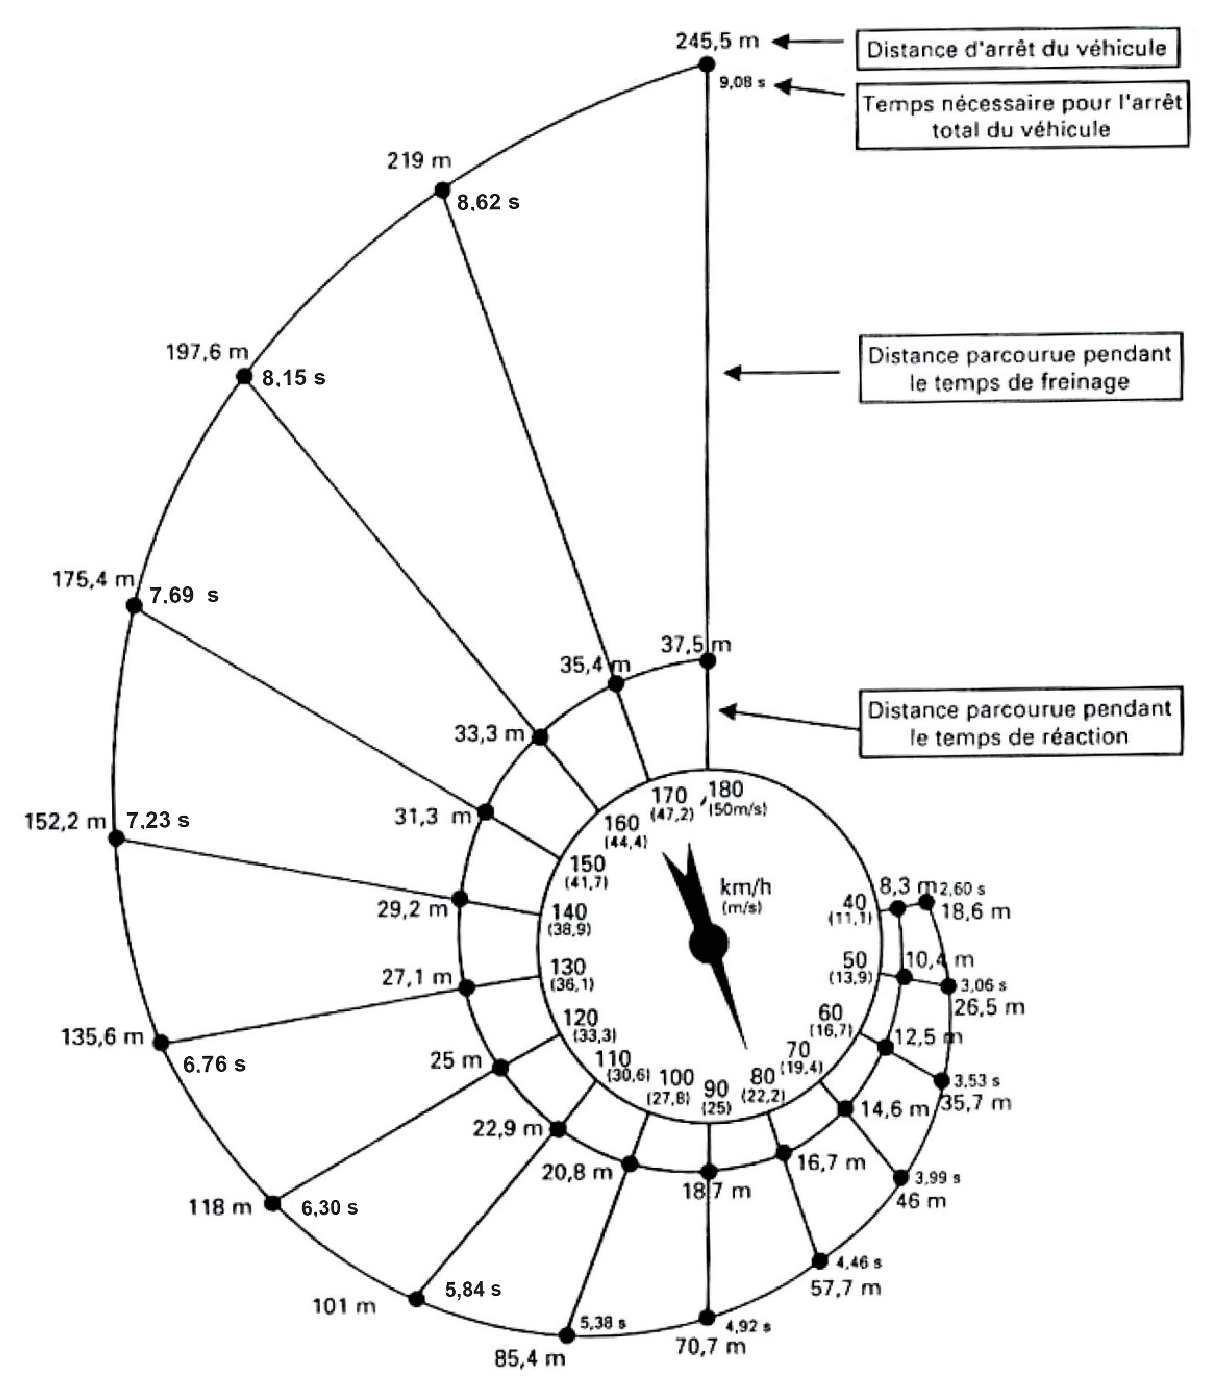
\includegraphics[width=15.cm]{Organisation_gestion_donnees/Images/D5_ex_escargot_arret}
         \end{center} \smallskip
         Par exemple, on peut lire que, pour une vitesse de 180 km/h (ou 50 m/s), un véhicule parcourt \um{37,5} pendant le temps de réaction, que le temps nécessaire à son arrêt total sera de \us{9,08}, et que sa distance d’arrêt sera alors de \um{245,5}. En utilisant ce diagramme,
   \begin{enumerate}
      \item donner la distance d’arrêt d’un véhicule roulant à 110 km/h ;
      \item donner la distance parcourue pendant le temps de freinage d’un véhicule roulant à 80 km/h ;
      \item donner le temps que met un véhicule roulant à 130 km/h pour s’arrêter ;
      \item donner la vitesse d’un véhicule sachant que la distance de réaction est de \um{25} ;
      \item dire si un conducteur roulant à 27,8 m/s et apercevant un obstacle à \um{100} pourra s’arrêter à temps. \\ [-8mm]
      \end{enumerate}
   \end{enumerate}
\end{exercice}

\begin{corrige}
\ \\ [-5mm]
   \begin{enumerate}
      \item Une vitesse de 90 km/h correspond à : $\dfrac{\um{90}}{\us{3600}} =25$ m/s. \\ [1mm]
         Sachant que la constante vaut $k =0,14$, en utilisant la formule donnée on obtient en mètre : \\
         $d_A =25\times0,75+0,14\times25^2 =106,25$. \\
         {\blue Un véhicule circulant sur route mouillée à 90 km/h mettra 106,25 mètres pour s'arrêter}. \\
      \item Pour un conducteur vigilant sur route sèche, on a $t_R =0,75$ et $k =0,14$, d'où : \\
   $d_A =0,75\,v+0,073\,v^2$. \\
          L'expression de la distance en fonction de la vitesse n'est pas une fonction linéaire à cause de la présence du \og $v^2$ \fg{} (il s'agit d'une fonction du second degré représentée par une parabole) donc, \\
         {\blue la distance d'arrêt sur route sèche n'est pas proportionnelle à la vitesse.}
   \item
      \begin{enumerate}
          \item Un véhicule roulant à 110 km/h s'arrête en {\blue \um{101}}.
          \item La distance de freinage à 80 km/h est de {\blue \um{41}}.
          \item Un véhicule qui roule à 130 km/h met {\blue \us{6,76}} pour s'arrêter.
          \item Un distance de réaction de \um{25} correspond à une vitesse de {\blue 120 km/h.}
          \item Un conducteur roulant à 27,8 m/s mettra \um{85,4} pour s'arrêter, donc {\blue il évitera l'obstacle}.
      \end{enumerate}
   \end{enumerate}
\end{corrige}

\bigskip


\begin{exercice}[CRPE 2006 G5] %%% 2
   \textit{Vu à la Cité des Sciences et de l'Industrie à Paris.} \\ [1mm] 
   Six réservoirs de formes différentes, de même volume, de même hauteur se remplissent dans le même temps. Il s'agit d'associer à une forme de récipient une jauge et une courbe indiquant la hauteur du liquide en fonction du temps sachant que :
   \begin{itemize}
      \item les graduations des six jauges A, B, C\dots{} indiquent les hauteurs de liquide correspondant à 1 litre, 2 litres\dots{} pour les six réservoirs ;
      \item les courbes 1, 2, 3\dots{} indiquent la hauteur atteinte par le liquide en fonction du temps lorsque les six réservoirs se remplissent ;
      \item les récipients ont tous le même volume 10 litres et la même hauteur. 
   \end{itemize}
   Leurs formes sont représentées grossièrement par les dessins ci-dessous. Pendant le remplissage, le débit de l'eau est constant et identique d'un récipient à l'autre. Ainsi, à un instant donné, le volume d'eau contenu dans chaque récipient est le même mais la hauteur d'eau n'est pas nécessairement la même.
   \begin{center}
   {\psset{unit=0.65}
      \begin{pspicture}(-0.5,-0.8)(2,3)
         \psline[linewidth=1.5pt](0,0)(2,0)
         \psline(0.65,3)(0.65,1.61)
         \psline(1.35,3)(1.35,1.61)
         \psarc(1,0.85){0.85}{114}{66} 
         \rput(1,-0.5){R1}
      \end{pspicture}
      \quad
      \begin{pspicture}(0,-0.8)(2,3)   
         \psline[linewidth=1.5pt](0,0)(2,0)
         \psline(0.5,3)(0.5,0)
         \psline(1.5,3)(1.5,0)
         \rput(1,-0.5){R2}
      \end{pspicture}
      \quad
      \begin{pspicture}(0,-0.8)(2,3)  
         \psline[linewidth=1.5pt](0,0)(2,0)
         \psline(0.75,0)(0.25,3)
         \psline(1.25,0)(1.75,3)
         \rput(1,-0.5){R3}
      \end{pspicture}
      \quad
      \begin{pspicture}(0,-0.8)(2,3) 
         \psline[linewidth=1.5pt](0,0)(2,0)
         \psarc(3.3,1.5){3}{150}{210} 
         \psarc(-1.3,1.5){3}{-30}{30}
         \rput(1,-0.5){R4}
      \end{pspicture}
      \quad
      \begin{pspicture}(0,-0.8)(2,3) 
         \psline[linewidth=1.5pt](0,0)(2,0)
         \psline(0.2,0)(0.8,1.5)(0.2,3)
         \psline(1.8,0)(1.2,1.5)(1.8,3)
         \rput(1,-0.5){R5}
      \end{pspicture}
      \quad
      \begin{pspicture}(0,-0.8)(2,3) 
         \psline[linewidth=1.5pt](0,0)(2,0)
         \psline(0.25,0)(0.75,3)
         \psline(1.75,0)(1.25,3) 
         \rput(1,-0.5){R6}
      \end{pspicture}}
      \hspace*{1.2cm}
      {\psset{xunit=0.4,yunit=0.3}
      \begin{pspicture}(0,0)(2,9)
         \psframe(0,0)(1,10)  
         \psline(0,1.7)(1,1.7)
         \psline(0,8.3)(1,8.3)
         \multido{\n=2.75+0.75}{7}{\psline(0,\n)(1,\n)} 
         \rput(0.5,-0.9){A}  
      \end{pspicture}
      \begin{pspicture}(0,0)(2,9)
         \psframe(0,0)(1,10)  
         \psline(0,0.2)(1,0.2)
         \psline(0,0.5)(1,0.5)
         \psline(0,1.3)(1,1.3)
         \psline(0,2.75)(1,2.75)
         \psline(0,5)(1,5)     
         \psline(0,7.25)(1,7.25)      
         \psline(0,8.7)(1,8.7)      
         \psline(0,9.5)(1,9.5)
         \psline(0,9.8)(1,9.8)
         \rput(0.5,-0.9){B}  
      \end{pspicture}
      \begin{pspicture}(0,0)(2,9)
         \psframe(0,0)(1,10)  
        \multido{\i=1+1}{9}{\psline(0,\i)(1,\i)} 
         \rput(0.5,-0.9){C}  
      \end{pspicture}
      \begin{pspicture}(0,0)(2,9)
      \psframe(0,0)(1,10)
         \psline(0,0.4)(1,0.4)
         \psline(0,0.85)(1,0.85)
         \psline(0,1.35)(1,1.35)
         \psline(0,1.95)(1,1.95)
         \psline(0,2.65)(1,2.65) 
         \psline(0,3.45)(1,3.45)    
         \psline(0,4.35)(1,4.35)   
         \psline(0,5.45)(1,5.45)
         \psline(0,6.85)(1,6.85)
         \rput(0.5,-0.9){D}  
      \end{pspicture}
      \begin{pspicture}(0,0)(2,9)
         \psframe(0,0)(1,10)  
         \psline(0,6.9)(1,6.9)
         \psline(0,5.4)(1,5.4)
         \multido{\n=2.2+0.4}{7}{\psline(0,\n)(1,\n)}
         \psline(0,1.5)(1,1.5)
         \rput(0.5,-0.9){E}  
      \end{pspicture}
      \begin{pspicture}(0,0)(1,9)
         \psframe(0,0)(1,10)  
         \psline(0,9.6)(1,9.6)
         \psline(0,9.15)(1,9.15)
         \psline(0,8.65)(1,8.65)
         \psline(0,8.05)(1,8.05)
         \psline(0,7.35)(1,7.35) 
         \psline(0,6.55)(1,6.55)    
         \psline(0,5.65)(1,5.65)    
         \psline(0,4.55)(1,4.55)
         \psline(0,3.15)(1,3.15)
         \rput(0.5,-0.9){F}  
      \end{pspicture}
      }
   \end{center}
   \begin{enumerate}
      \item Associer à chaque récipient R1, R2, R3, R4, R5, R6 :
      \begin{enumerate}
         \item la jauge qui lui correspond parmi les jauges A, B, C, D, E, F reproduites ci-dessus ;
         \item la courbe qui lui correspond parmi les courbes 1, 2, 3, 4, 5, 6 reproduites ci-dessous. Présenter les résultats dans un tableau, sans justification.
         \begin{multicols}{3}
         {\psset{unit=0.3}
            \begin{pspicture}(0,0)(15,10)
               \multido{\i=0+1}{16}{\psline[linecolor=gray](\i,0)(\i,10)}
               \multido{\i=0+1}{11}{\psline[linecolor=gray](0,\i)(15,\i)} 
               \psline[linewidth=1.5pt](0,0)(15,10)
               \rput(1.5,8.5){\Large1}
            \end{pspicture} \\        
            \begin{pspicture}(0,2)(15,12)
               \multido{\i=0+1}{16}{\psline[linecolor=gray](\i,0)(\i,10)}
               \multido{\i=0+1}{11}{\psline[linecolor=gray](0,\i)(15,\i)} 
               \psarc[linewidth=1.5pt](2.8,-0.9){3}{125}{163}
               \psline[linewidth=1.5pt](1,1.5)(14,8.5)
               \psarc[linewidth=1.5pt](12.2,10.9){3}{306}{342}
               \rput(1.5,8.5){\Large4}
            \end{pspicture} \\            
            \begin{pspicture}(0,0)(15,10)
               \multido{\i=0+1}{16}{\psline[linecolor=gray](\i,0)(\i,10)}
               \multido{\i=0+1}{11}{\psline[linecolor=gray](0,\i)(15,\i)} 
               \psarc[linewidth=1.5pt](2.95,-0.85){3}{107}{163}
               \psline[linewidth=1.5pt](2,2)(12,5)
               \psarc[linewidth=1.5pt](11.05,7.85){3}{287}{344}
               \psline[linewidth=1.5pt](13.95,7)(15,10)
               \rput(1.5,8.5){\Large2}
            \end{pspicture} \\            
            \begin{pspicture}(0,2)(15,12)
               \multido{\i=0+1}{16}{\psline[linecolor=gray](\i,0)(\i,10)}
               \multido{\i=0+1}{11}{\psline[linecolor=gray](0,\i)(15,\i)} 
               \psecurve[linewidth=1.5pt](-0.1,-20)(0,0)(1,2.5)(5,6)(9,8)(15,10)(17,10.2)
               \rput(1.5,8.5){\Large5}
            \end{pspicture} \\            
            \begin{pspicture}(0,0)(15,10)
               \multido{\i=0+1}{16}{\psline[linecolor=gray](\i,0)(\i,10)}
               \multido{\i=0+1}{11}{\psline[linecolor=gray](0,\i)(15,\i)} 
               \psecurve[linewidth=1.5pt](-2,-0.2)(0,0)(6,2)(10,4)(14,7.5)(15,10)(15.1,30)
               \rput(1.5,8.5){\Large3}
            \end{pspicture} \\                     
            \begin{pspicture}(0,2)(15,12)
               \multido{\i=0+1}{16}{\psline[linecolor=gray](\i,0)(\i,10)}
               \multido{\i=0+1}{11}{\psline[linecolor=gray](0,\i)(15,\i)} 
               \psarc[linewidth=1.5pt](0.04,8.1){8.08}{270}{338}
               \psarc[linewidth=1.5pt](14.96,1.9){8.08}{90}{158}
               \rput(1.5,8.5){\Large6}
            \end{pspicture}}            
         \end{multicols}
      \end{enumerate}
      \smallskip
      \item Sachant que le diamètre du récipient cylindrique R2 est de 16 cm, calculer la hauteur de ce récipient (arrondie au centimètre).
      \item À un instant $t$, le récipient cylindrique R2 est rempli aux 2/3 de sa hauteur. Calculer, au dixième de litre près, le volume d'eau $\mathcal{V}'$ contenu dans le cylindre à cet instant précis.
      \item On observe la hauteur d'eau dans le récipient R6 au moment où le récipient cylindrique R2 est rempli aux 2/3 de sa hauteur. Est-elle plus ou moins haute que dans R2 ? Justifier la réponse en utilisant les courbes ci-dessus.
   \end{enumerate}    
\end{exercice}

\begin{corrige}
\ \\ [-2.5mm]
\begin{enumerate}
   \item
      \begin{LCtableau}{0.7\linewidth}{7}{c}
         \hline
         Récipient & R1 & R2 & R3 & R4 & R5 & R6 \\
         \hline
         Jauge & \textcolor{blue}{E} & \textcolor{blue}{C} & \textcolor{blue}{F} & \textcolor{blue}{A} & \textcolor{blue}{B} & \textcolor{blue}{D} \\
         \hline
         Courbe & \textcolor{blue}{2} & \textcolor{blue}{1} & \textcolor{blue}{5} & \textcolor{blue}{4} & \textcolor{blue}{6} & \textcolor{blue}{3} \\
         \hline
      \end{LCtableau}
   \item Le volume d'un cylindre de hauteur $h$ et de rayon de base $r$ est : $\mathcal{V} =\pi\times r^2\times h$. \\
      Le diamètre de R2 est de 16 cm, donc son rayon vaut 8 cm ; \\
      le volume est de 10 litres, soit \udmc{10}, ou encore \ucmc{10000}. On a alors : \\
      $\ucmc{10000} =\pi\times 8^2\times \Ucmc{h} \iff h =\dfrac{\ucmc{10000}}{\Ucmq{64\pi}} \approx\ucm{49,74}$. \\ [1mm]
      {\blue Le récipient R2 mesure environ 50 centimètres de haut.}  
   \item Le cylindre R2 se remplit de manière homogène, donc, $\mathcal{V}' =\dfrac23\times\mathcal{V} =\dfrac23\times10\,\text{L} \approx 6,67$ L. \\
   {\blue À l'instant $t$, le récipient R2 contient environ 6,7 litres d'eau.}  
   \item La courbe correspondant à R2 est la courbe 1 : c'est une fonction linéaire puisque le débit est constant. \\
   Sur l'axe des abscisses, 15 carreaux représentent le temps pour remplir les réservoirs en entier, donc 10 carreaux représentent les deux tiers du temps $\left(\dfrac23\times15 =10\right)$. \\
   À cet endroit, la courbe représentative de R2 est au dessus de la courbe représentative de R6 d'où : \\
   {\blue aux deux tiers du temps, la hauteur d'eau dans le récipient R2 est supérieure à celle du récipient R6.}
\end{enumerate}    
\end{corrige}

\bigskip


\begin{exercice}[CRPE 2021 G1] %%% 6
   L’entreprise AMP’OUL travaille avec deux sociétés de livraison, qui lui proposent des tarifs adaptés à ses besoins.
   \begin{center}
      {\hautab{1.5}
      \begin{tabular}{|C{3}|C{3}|C{3}|}
         \hline
         Société & Tarif par palette (\euro) & Frais de gestion (\euro) \\
         \hline
         Société A & 12 & 284 \\
         \hline
         Société B & 29 & 115 \\
         \hline
      \end{tabular}}
   \end{center}
   On définit les fonctions $f$ et $g$ par les expressions algébriques suivantes :
   \begin{itemize}
      \item $f(x) =12x+284$
      \item $g(x) =29x+115$
   \end{itemize}
   Ainsi, si $x$ désigne un nombre de palettes alors $f(x)$ et $g(x)$ désignent respectivement le prix à payer pour la livraison de ces $x$ palettes par les sociétés A et B. \\
   On a tracé les courbes correspondant à $f$ et $g$ dans le repère ci-dessous.
   \begin{center}
      {\psset{unit=0.9}
      \small
      \begin{pspicture}(-1,-0.3)(16.5,11.5)
         \psgrid[subgriddiv=0, gridlabels=0pt, gridcolor=gray!60](0,0)(16,11)
         \psaxes[dy=1,Dy=50]{->}(0,0)(16.3,11.3)
         \psline(0,2.3)(15,11)
         \psline(0,5.68)(16,9.52)
         \rput(1.5,6.5){$C_1$}
         \rput(1.5,2.5){$C_2$}
         \rput(14,0.5){Nombre de palettes}
         \rput(1,10.5){Prix (\euro)}
      \end{pspicture}}
   \end{center}
   \begin{enumerate}
      \item Répondre, en vous aidant du graphique, aux questions suivantes :
         \begin{enumerate}
            \item Identifier la courbe qui correspond à chaque fonction.
            \item Quelle société de livraison sera la plus économique pour une commande de 6 palettes ?
            \item Pour une commande donnée, quelle société de livraison sera la plus économique en fonction du nombre de palettes ?
         \end{enumerate}
      \item Résoudre l’équation $f(x) =g(x)$. Utiliser cette résolution pour affiner la réponse à la question 1.c.
   \end{enumerate}
\end{exercice}

\begin{corrige}
\ \\ [-5mm]
   \begin{enumerate}
      \item 
         \begin{enumerate}
            \item Les deux fonctions sont affines, donc représentées par des droites. On peut lire l'ordonnée à l'origine de chacune des droites : 
               \begin{itemize}
                  \item l'ordonnée à l'origine de $f$ vaut 284, qui correspond à l'ordonnée à l'origine de la droite $C_1$ ;
                  \item l'ordonnée à l'origine de $g$ vaut 115, qui correspond à l'ordonnée à l'origine de la droite $C_2$.
               \end{itemize}
               {\blue La fonction $f$ est représentée par la courbe $C_1$ et $g$ par $C_2$}.
            \item Pour 6 palettes, c'est la courbe $C_2$ qui a l'ordonnée la plus petite, donc la fonction $g$, ce qui correspond à {\blue la société B}.
            \item Graphiquement, la courbe représentative de $g$ est située en dessous de celle de $f$ pour un nombre de palettes inférieur à 10. Donc, {\blue entre 0 et 9 palettes, il est préférable de choisir la société B, et à partir de 10 palettes il vaut mieux choisir la société A}.   
         \end{enumerate}
      \setcounter{enumi}{1}
      \item $f(x) =g(x) \iff 12x+284 =29x+115$ \\
         \hspace*{2.13cm} $\iff 284-115 =29x-12x$ \\
         \hspace*{2.13cm} $\iff 169 =17x$ \\ [1mm]
         \hspace*{2.13cm} $\iff {\blue x =\dfrac{169}{17}} x \approx9,94$ \\ [1mm]
         $x$ étant un nombre entier, {\blue la société B est bien préférable pour un nombre de palettes compris entre 0 et 9}.
      \end{enumerate}
\end{corrige}

\bigskip


\begin{exercice}[CRPE 2018 G2] %%% 1
   On s’intéresse à la réalisation d’une canette en forme de cylindre de révolution de base de rayon $r$, exprimé en centimètre, et de contenance \ucl{33}. L’aire, exprimée en centimètre carré, de la surface de métal nécessaire est modélisée par la fonction $f$ qui, à tout nombre $r$ strictement positif, associe $f(r) =2\pi r^2+\dfrac{660}{r}$.
   \begin{enumerate}
      \item La fonction $f$ est représentée ci-dessous : \smallskip
         \begin{center}
         \psset{unit=0.58,algebraic=true}
            \begin{pspicture*}(-1.5,-1)(22,14)
               \psgrid[subgriddiv=0,gridlabels=0pt,gridcolor=gray!60](0,0)(21,14)
               \psaxes[dy=1,Dy=50,dx=1,Dx=0.5,labelFontSize=\scriptstyle,comma=true]{->}(21,14)
               \psplot{0.5}{21}{Pi*x^2/100+132/(5*x)}
            \end{pspicture*}
         \end{center}
         Répondre par lecture graphique aux questions suivantes :
        \begin{enumerate}
            \item Quelle est l’aire de la surface de métal nécessaire pour un cylindre dont la base a pour rayon \ucm{1,5} ?
            \item À quelle(s) valeur(s) du rayon du cylindre correspond une aire de \ucmq{300} ?
            \item Une canette classique a un diamètre de \ucm{6,6} et une canette slim a un diamètre de \ucm{5,6}. Déterminer laquelle de la canette classique ou de la canette slim utilise le moins de surface de métal pour sa réalisation. Justifier la réponse en donnant les lectures graphiques effectuées.
            \item À quelle valeur du rayon correspond la surface minimale de métal nécessaire à la fabrication d’une canette de \ucl{33} ?
         \end{enumerate}
      \item Voici une copie d’écran de la feuille de calcul relative à $f$.
         \begin{center}
         \texttt{\hautab{1.5}\small
            \begin{tabular}{|>{\columncolor{lightgray!30}}c|*{13}{C{0.9}|}}
               \hline
              \rowcolor{lightgray!30} & A & B & C & D & E & F & G & H & I & J & K & L \\
               \hline
               1 & $r$ & 3 & 3,1 & 3,2 & 3,3 & 3,4 & 3,5 & 3,6 & 3,7 & 3,8 & 3,9 & 4 \\
               \hline
               2 & $f(r)$ & 276,55 & 273,28 & 270,59 & 268,42 & 266,75 & 265,54 & 264,76 & 264,40 & 264,41 & 264,80 & 265,63 \\
               \hline
            \end{tabular}}
         \end{center}
         \begin{enumerate}
            \item Écrire une formule qui, entrée dans la cellule B2 et étirée vers la droite, permet d’obtenir les valeurs de $f(r)$ sur la ligne 2. {\it Note : la fonction \texttt{PI()} du tableur renvoie la valeur de $\pi$ avec une précision de 15 décimales.}
            \item Utiliser cette feuille de calcul pour déterminer un encadrement, le plus précis possible, du rayon du cylindre permettant de minimaliser l’aire de la surface de métal nécessaire à la réalisation d’une canette de 33 cL.
         \end{enumerate}
   \end{enumerate}
\end{exercice}

\begin{corrige}
\ \\ [-5mm]
   \begin{enumerate}
      \item
         \begin{enumerate}
            \item Pour l'abscisse $r =\ucm{1,5}$, on lit une aire environ égale à {\blue \ucmq{450}}.
            \item Pour une ordonnée $\mathcal{A} =\ucmq{300}$, on lit deux valeurs pour le rayon : {\blue $r_1 \approx\ucm{2,5}$ et $r_2 \approx \ucm{5,25}$}.
            \item Pour une canette classique de rayon \ucm{3,3}, on lit une aire d'environ \ucmq{270} et pour une canette slim de rayon \ucm{2,8}, on lit une aire d'environ \ucmq{285}. Donc, {\blue c'est la canette classique qui demande le moins de surface de métal}.
            \item La surface minimale est atteinte pour un rayon d'environ {\blue \ucm{3,75}}.
         \end{enumerate}
      \setcounter{enumi}{1}
      \item
         \begin{enumerate}
            \item Dans \texttt{B2}, on peut écrire : {\blue \texttt{=2*PI()*B1$\wedge$2+660/B1}}
            \item Les valeurs minimales pour l'aire dans le tableau sont 264,40 et 264,41, elles correspondent à \\
   {\blue un rayon compris entre 3,7 cm et 3,8 cm.}
         \end{enumerate}
   \end{enumerate}
\end{corrige}

\bigskip


\begin{exercice}[Bon de commande] %%%1
   Un laboratoire d'analyses souhaite passer des commandes de bureautique auprès d'une centrale d'achat. Construire sur tableur le bon de commande ci-dessous.
   \begin{center}
   \texttt{
   {\hautab{1.6}
      \begin{tabular}{|>{\columncolor{lightgray!30}}p{0.4cm}|p{3cm}|C{3}|C{3}|C{3}|}
         \hline
         \rowcolor{lightgray!30} & \centering A & B & C & D \\
         \hline
        1 & Bon de commande & & & \\
         \hline
         2 & & & & \\
         \hline
         3 & \cellcolor{FondTableaux}{Désignation de l'article} & \cellcolor{FondTableaux}{Quantité} & \cellcolor{FondTableaux}{Prix unitaire HT (en \euro)} & \cellcolor{FondTableaux}{Total} \\
         \hline
         4 & Fauteuil & 5 & 295,90 & \\
         \hline
         5 & Bureau & 5 & 139,50 & \\
         \hline
         6 & Caisson à tiroirs & 4 & 139,00 & \\
         \hline
         7 & Ordinateur & 4 & 389,80 & \\
         \hline
         8 & Armoire & 2 & 269,00 & \\
         \hline
         9 & Bibliothèque & 4 & 129,90 & \\
         \hline
         10 & & & & \\
         \hline
         11 & & & Prix HT & \\
         \hline
         12 & Taux de remise & & Remise & \\
         \hline
         13 & Taux de TVA & 19,60\,\% & Montant TVA & \\
         \hline
         14 & & & & \\
         \hline
         15 & & & Prix total & \\
         \hline
      \end{tabular}}
   }
   \end{center}
   \begin{enumerate}
      \item Entrer une formule en D4 puis la recopier jusqu'en D9 pour obtenir le total en euros de chaque article.
      \item Proposer une formule à entrer en D11 permettant de calculer le prix total hors taxe.
      \item Le taux de remise accordé par la centrale d'achat est de 5\% ou 10\% sur le prix hors taxe.
Entrer en B12 la formule \cell{=SI(D11<5000;0,05;0,10)}. À quoi correspond cette formule ?
      \item Donner une formule à entrer en D12 permettant de calculer le montant de la remise.
      \item Peut-on recopier vers le bas en D13 le contenu de la cellule D12, pour obtenir la somme en euros correspondant à la TVA calculée sur le prix hors taxe avant remise ? Calculer cette somme en D13.
      \item Entrer en D15 une formule donnant le prix total à payer.
      \item Quelles modifications apparaissent sur le bon de commande si le laboratoire d'analyses modifie sa commande en ne commandant plus que trois ordinateurs ? Quel est alors le prix total à payer ?
   \end{enumerate}
   \hfill {\it\small Source : \url{http://mechain.lyc.ac-amiens.fr/spip_pead/IMG/pdf/module-tableur-pourcentages.pdf}}
\end{exercice}

\begin{corrige}
\ \\ [-5mm]
   \begin{enumerate}
      \item En D4, on entre : {\blue\texttt{=B4*C4}}
      \item en D11, on entre : {\blue\texttt{=SOMME(D4:D9)}}
      \item Cette formule est une formule conditionnelle : si le total HT est inférieur à 5 000 \euro, la remise sera de 5\,\% (0,05), sinon, la remise sera de 10\,\% (0,10).
      \item En D12, on entre {\blue\texttt{=D11*B12}}
      \item Non, car sinon, le calcul de la TVA se ferait sur la remise. En D13, on entre {\blue\texttt{=D11*B13}} \\
   Remarque : la recopie aurait été possible si on avait fixé la cellule D11, au moins au niveau de la ligne avec par exemple la formule {\blue\texttt{=D\$11*B12}} 
      \item En D15, on entre {\blue\texttt{=D11-D12+D13}}
      \item Si on réduit le nombre d'ordinateurs à 3, les cellules suivantes changent : D7 (somme payée pour les ordinateurs), D11 (prix HT), B12 (pourcentage de la remise), D12 (remise), D13 (montant de la TVA) et D15 (prix total). Le prix à payer est de {\blue \ueuro{5 684,16}}.
   \end{enumerate}
\end{corrige}

\bigskip


\begin{exercice}[CRPE 2019 G1] %%%2
   Les figures ci-dessous -- qui ne sont pas nécessairement à l’échelle -- représentent quatre carrés dont les mesures des côtés, en centimètre, sont des nombres entiers consécutifs.
   \begin{center}
      {\psset{unit=0.5}
      \begin{pspicture}(0,-1)(11,4)
         \psframe[fillstyle=solid,fillcolor=gray!60](0,0)(1,1)
         \psframe(1,0)(3,2)
         \psframe(3,0)(6,3)
         \psframe[fillstyle=solid,fillcolor=gray!60](6,0)(10,4)
         \rput(5,-1){\it cas 1}
      \end{pspicture}
      \qquad
      \begin{pspicture}(0,-1)(10,4)
         \psframe[fillstyle=solid,fillcolor=gray!60](0,0)(1,1)
         \psframe[fillstyle=solid,fillcolor=gray!60](1,0)(3,2)
         \psframe[fillstyle=solid,fillcolor=gray!60](3,0)(6,3)
         \psframe(6,0)(10,4)
         \rput(5,-1){\it cas 2}
      \end{pspicture}}
   \end{center}
   On cherche à savoir si, dans chacun de ces cas, ill est possible que l’aire de la surface grise soit égale à l’aire de la surface blanche. \\
   On utilise pour cela un tableur. On donne ci-dessous les copies d’écran des feuilles de calcul obtenues lors de cette recherche.
   \begin{center}
      \texttt{\small
      \begin{tabular}{|>{\columncolor{lightgray!30}}c|*{7}{C{1.8}|}}
         \hline
         \rowcolor{lightgray!30} & A & B & C & D & E & F & G \\
         \hline
         1 & côté du petit carré & aire du 1er carré & aire du 2ème carré & aire du 3ème carré & aire du 4ème carré & aire partie grise & aire partie blanche \\
         \hline
         2 & 1 & 1 & 4 & 9 & 16 & 17 & 13 \\
         \hline
         3 & 50 & 2500 & 2601 & 2704 & 2809 & 5309 & 5305 \\
         \hline
         4 & 100 & 10000 & 10201 & 10404 & 10609 & 20609 & 20605 \\
         \hline
         5 & 700 & 490000 & 491401 & 492804 & 494209 & 984209 & 984205 \\
         \hline
         6 & 1000 & 1000000 & 1002001 & 1004004 & 1006009 & 2006009 & 2006005 \\
         \hline  
         7 & 2000 & 4000000 & 4004001 & 4008004 & 4012009 & 8012009 & 8012005 \\
         \hline
         8 & 50000 & 2500000000 & 2500100001 & 2500200004 & 2500300009 & 5000300009 & 5000300005 \\
         \hline
         9 & 100000 & 10000000000 & 10000200001 & 10000400004 & 10000600009 & 20000600009 & 20000600005 \\
         \hline
      \end{tabular}} \\ [1mm]
      {\it Feuille de calcul A} \\ [5mm]   
      \texttt{\small
      \begin{tabular}{|>{\columncolor{lightgray!30}}c|*{7}{C{1.8}|}}
         \hline
         \rowcolor{lightgray!30} & A & B & C & D & E & F & G \\
         \hline
         1 & côté du petit carré & aire du 1er carré & aire du 2ème carré & aire du 3ème carré & aire du 4ème carré & aire partie grise & aire partie blanche \\
         \hline
         2 & 1 & 1 & 4 & 9 & 16 & 14 & 16 \\
         \hline
         3 & 2 & 4 & 9 & 16 & 25 & 29 & 25 \\
         \hline
         4 & 3 & 9 & 16 & 26 & 36 & 50 & 36 \\
         \hline
         5 & 4 & 16 & 25 & 36 & 49 & 77 & 49 \\
         \hline
         6 & 5 & 25 & 36 & 49 & 64 & 110 & 64 \\
         \hline
         7 & 6 & 36 & 49 & 64 & 81 & 149 & 81 \\
         \hline
         8 & 7 & 49 & 64 & 81 & 100 & 194 & 100 \\
         \hline
         9 & 8 & 64 & 81 & 100 & 121 & 245 & 121 \\
         \hline 
      \end{tabular}} \\ [1mm]
      {\it Feuille de calcul B}
   \end{center}
   \begin{enumerate}
      \item Quelle feuille correspond à chacun des deux cas ? Justifier la réponse.
      \item Pour la feuille de calcul A :
         \begin{enumerate}
            \item Quelle formule étirable vers le bas a-t-on pu saisir dans la cellule E2 pour calculer l’aire du quatrième carré à partir de la valeur saisie dans la cellule A2 ?
            \item Quelle formule étirable vers le bas a-t-on pu saisir dans la cellule F2 pour calculer l’aire de la partie grise ?
         \end{enumerate}
      \item Pour chaque cas, quelle conjecture, sur les solutions du problème, la copie d’écran de la feuille de calcul permet-elle d’émettre ? Justifier la réponse.
      \item Démontrer que dans less deux cas, le problème n’admet pas de solution.
   \end{enumerate}
\end{exercice}

\begin{corrige}
\ \\ [-5mm]
   \begin{enumerate}
      \item Pour le cas 1, l'aire de la partie blanche est égale à la somme des aires des carrés 2 et 3. Il suffit donc de regarder dans quelle feuille de calcul c'est également le cas en regardant les valeurs des colonnes C, D et G : \\
         Pour la feuille A, en ligne 2, on a $4 + 9$ qui est bien égal à 13. \\
         Pour la feuille B, en ligne 2, on a $4 + 9$ qui n'est pas égal à 16. \\
        {\blue La feuille de calcul A correspond au cas 1 et la feuille B correspond au cas 2}.
      \item
         \begin{enumerate}
            \item En E2, on a pu saisir la formule : {\blue \texttt{=(A2+3)$\wedge$2}}
            \item En F2, on a pu saisir la formule : {\blue \texttt{=B2+E2}}
         \end{enumerate}
      \setcounter{enumi}{2}
      \item -- Pour la feuille de calcul A, on remarque que la valeur de chaque cellule de la colonne F est augmentée de 4 par rapport à sa cellule voisine de la colonne G, et si cela se vérifie pour toutes les valeurs, alors les deux aires ne pourront jamais être égales. \\
         -- Pour la feuille de calcul B, les valeurs des cellules de la colonne F augmentent plus vite que celles de la colonne G tout en étant supérieures à partir de 2. Pour 1, les aires ne sont pas égales et comme les valeurs des côtés sont des nombres entiers naturels, il semble impossible de trouver une solution au problème. \\
      {\blue D'après les copies d'écran, on peut conjecturer qu'il n'y a aucune solution au problème quelle que soit la configuration}.
   \item On appelle $n$ la mesure, en centimètre, du côté du carré le plus petit.
      \begin{itemize}
         \item Le cas 1 se modélise par l'équation suivante : \\
            $n^2+(n+3)^2 =(n+1)^2+(n+2)^2 \iff \cancel{n^2}+\cancel{n^2}+6n+9 =\cancel{n^2}+2n+1+\cancel{n^2}+4n+4$ \\
            \hspace*{4.95cm} $\iff \cancel{6n}+9 =\cancel{6n}+5$ \\
            \hspace*{4.95cm} $\iff 9 =5$. Cette équation n'est donc pas possible.
         \item Le cas 2 se modélise par l'équation suivante : \\
            $n^2+(n+1)^2+(n+2)^2 =(n+3)^2 \iff \cancel{n^2}+n^2+2n+1+n^2+4n+4 =\cancel{n^2}+6n+9$ \\
            \hspace*{4.95cm} $\iff 2n^2+\cancel{6n}+5 =\cancel{6n}+9$ \\
            \hspace*{4.95cm} $\iff 2n^2 =4$ \\
            \hspace*{4.95cm} $\iff n^2 =2$. Les solutions de cette équation sont $\sqrt2$ et $-\sqrt2$ qui ne sont pas des nombres entiers, donc le cas 2 n'a pas de solution.
      \end{itemize}
      Conclusion : {\blue Cette situation n'a pas de solution}.
   \end{enumerate}
\end{corrige}

\bigskip


\begin{exercice}[CRPE 2016 G2] %%%3
   Les télésièges sont équipés de véhicules fixés à un câble. Sur un télésiège donné, tous les véhicules ont le même nombre de sièges, généralement compris entre deux et six. Pour des raisons de sécurité, l'espacement minimal entre deux véhicules sur le câble dépend de la vitesse de déplacement des véhicules et du nombre de sièges par véhicule selon la formule ci-dessous, valable pour un nombre de sièges inférieur ou égal à six : $E =V\left(4+\dfrac{n}{2}\right)$ où $E$ désigne l'espacement minimal en mètre ; $V$ désigne la vitesse des véhicules en mètre par seconde et n désigne le nombre de sièges par véhicule. La feuille de tableur page suivante a été créée en vue de calculer l'espacement minimal entre deux véhicules d'un télésiège, dans la suite de l'exercice on considère que l'espacement entre les véhicules est l'espacement minimal ainsi calculé.
   \begin{enumerate}
      \item La cellule E13 contient la valeur 18. Interpréter cette valeur dans le contexte de l'exercice.
      \item Choisir une formule parmi celles données ci-dessous qui peut être saisie en E3 puis étirée vers le bas pour calculer l'ensemble des valeurs de la colonne E. \medskip
      \begin{center}
         {\hautab{1.3}
         \begin{tabular}{|p{3cm}|p{3cm}|p{3cm}|}
            \hline
            \texttt{=\$B3*(4+E\$2/2)} & \texttt{=2*(4+4/2)} & \texttt{=12} \\
            \hline
            \texttt{=B3*(4+E2/2)} & \texttt{=B3*(4+4/2)} & \texttt{=\$B\$3*(4+\$E\$2/2)} \\
            \hline
         \end{tabular}
         }
      \end{center} \smallskip
      \item Le débit $D$ en nombre de personnes par heure est fourni par la formule : $D =3\,600\,n\dfrac{V}{E}$. \\
         L'affirmation suivante est-elle cohérente avec les données de cet exercice? \\
         \og {\it Les télésièges fabriqués en 2010 sont généralement équipés de véhicules à quatre places, avec une vitesse de ligne de 2,3~m/s et peuvent, au maximum, atteindre un débit de 2 400 personnes par heure.} \fg
      \item Pour des véhicules à quatre sièges, une vitesse de 2~m/s fournira-t-elle un meilleur débit qu'une vitesse de 3~m/s? (on se placera dans le cadre d'un espacement minimal dans chaque situation).
      \item Montrer que, dans le cas où on choisit l'espacement minimal en fonction de la vitesse, le débit peut s'exprimer uniquement en fonction du nombre de sièges par véhicule. Cela confirme-t-il le résultat trouvé à la question 4 ?
   \end{enumerate}
    \begin{center}
      \texttt{
         \begin{tabular}{|>{\columncolor{lightgray!30}}p{0.4cm}|*{8}{C{1.2}|}}
            \hline
            \rowcolor{lightgray!30} & A & B & C & D & E & F & G & H \\
            \hline 
            1 & & & \multicolumn{5}{c|}{Nombre de sièges par véhicules} & \\     
            \hline
            2 & & \cellcolor{FondTableaux}{Vitesse} & \cellcolor{FondTableaux}{2} & \cellcolor{FondTableaux}{3} & \cellcolor{FondTableaux}{4} & \cellcolor{FondTableaux}{5} & \cellcolor{FondTableaux}{6} & \\
            \hline
            3 & & 2 & 10 & 11 & 12 & 13 & 14 & \\
            \hline
            4 & & 2,1 & 10,5 & 11,55 & 12,6 & 13,65 & 14,7 & \\
            \hline
            5 & & 2,2 & 11 & 12,1 & 13,2 & 14,3 & 15,4 & \\
            \hline
            6 & & 2,3 & 11,5 & 12,65 & 13,8 & 14,95 & 16,1 & \\
            \hline
           7 & & 2,4 & 12 & 13,2 & 14,4 & 15,6 & 16,8 & \\
            \hline
            8 & & 2,5 & 12,5 & 13,75 & 15 & 16,25 & 17,5 & \\
            \hline
            9 & & 2,6 & 13 & 14,3 & 15,6 & 16,9 & 18,2 & \\
            \hline
            10 & & 2,7 & 13,5 & 14,85 & 16,2 & 17,55 & 18,9 & \\
            \hline
            11 & & 2,8 & 14 & 15,4 & 16,8 & 18,2 & 19,6 & \\
            \hline
            12 & & 2,9 & 14,5 & 15,95 & 17,4 & 18,85 & 20,3 & \\
            \hline
            13 & & 3 & 15 & 16,5 & 18 & 19,5 & 21& \\
            \hline
            14 & & 3,1 & 15,5 & 17,05 & 18,6 & 20,15 & 21,7 & \\
            \hline
            15 & & 3,2 & 16 & 17,6 & 19,2 & 20,8 & 22,4 & \\
            \hline
            16 & & 3,3 & 16,5 & 18,15 & 19,8 & 21,45 & 23,1 & \\
            \hline
            17 & & 3,4 & 17 & 18,7 & 20,4 & 22,1 & 23,8 & \\
            \hline
            18 & & 3,5 & 17,5 & 19,25 & 21 & 22,75 & 24,5 & \\
            \hline
         \end{tabular}
      }
      \end{center}
\end{exercice}
   
\begin{corrige}
\ \\ [-5mm]
   \begin{enumerate}
      \item La valeur 18 correspond à {\blue l'espacement minimal en mètre entre deux véhicules à une vitesse de 3 m/s pour 4 sièges par véhicule}.
      \item On peut choisir les formules suivantes : {\blue\texttt{=\$B3*(4+E\$2/2)}} ou {\blue\texttt{=B3*(4+4/2)}}
      \item La cellule E3 nous indique que, pour un véhicule à 4 places se déplaçant à 2,3 m/s, l'espacement minimal est de \um{13,8}. Avec la formule, on obtient alors : $D =3\,600\times4\times\dfrac{2,3}{13,8} =2\,400$. \\ [1mm]
         {\blue L'affirmation est cohérente avec les données de l'énoncé}.
      \item -- La cellule E6 nous indique que, pour un véhicule à 4 places se déplaçant à 2 m/s, l'espacement minimal est de \um{12}. Avec la formule, on obtient alors : $D =3\,600\times4\times\dfrac{2}{12} =2\,400$. \\ [1mm]
         -- La cellule E13 nous indique que, pour un véhicule à 4 places se déplaçant à 3 m/s, l'espacement minimal est de \um{18}. Avec la formule, on obtient alors : $D =3\,600\times4\times\dfrac{3}{18} =2\,400$. \\ [1mm]
         {\blue Pour des véhicules à 4 sièges, le débit est identique que la vitesse soit de 2~m/s ou de 3~m/s}. \smallskip
      \item On a $D =3\,600\,n\dfrac{V}{E}$ où $E =V\left(4+\dfrac{n}{2}\right)$ soit $\dfrac{E}{V} =4+\dfrac{n}{2}$ \\ [1mm]
         En prenant l'inverse de cette expression, on obtient $\dfrac{V}{E} =\dfrac{1}{4+\dfrac{n}{2}}$. \\ [1mm]
         Alors, $D =\dfrac{3\,600\,n}{4+\dfrac{n}{2}} =\dfrac{7\,200\,n}{8+n}$. \\ [1mm]
         {\blue Le débit $D$ s'exprime donc uniquement en fonction du nombre de sièges $n$}. \\
         Ce qui confirme le résultat trouvé dans la question 4 : en effet, avec $n=4$, on trouve $D =\dfrac{7\,200\times4}{8+4} =2\,400$.
   \end{enumerate}
\end{corrige}

\bigskip


\begin{exercice}[CRPE 2020 G1] %%%4
   Un fabricant de sauce tomate doit produire des boîtes de conserve cylindriques de volume fixé \ucmc{908}. Il souhaite minimiser le coût du métal, pour cela il cherche à minimiser l’aire totale $\mathcal{A}$ de la boîte ; celle-ci correspond à la somme de l’aire des disques de base et de l’aire de la surface latérale du cylindre. Il étudie l’évolution de l’aire de métal totale $\mathcal{A}$, en centimètre carré, en fonction du rayon $r$, en centimètre, du disque de base.
   \begin{enumerate}
      \item Dessiner à main levée un patron d’une boîte de conserve cylindrique en repassant de la même couleur les éléments de même longueur.
      \item Sachant que le volume de la boîte est de \ucmc{908}, donner l’expression de la hauteur $h$, exprimée en centimètre, de la boîte en fonction du rayon $r$.
      \item Pour calculer l’aire totale des cylindres de rayons différents, on a construit à l’aide d’un tableur la feuille de calcul suivante : \smallskip
         \begin{center}
         \texttt{\small\hautab{1.25}
            \begin{tabular}{|>{\columncolor{lightgray!30}}p{0.4cm}|*{5}{C{2}|}}
               \hline
               \rowcolor{lightgray!30} & A & B & C & D & E \\
               \hline 
               1 & Rayon $r$ (cm) & Hauteur $h$ (cm) & Aire d'un disque de base (\ucmq{}) & Aire latérale (\ucmq{}) & Aire totale du cylindre (\ucmq{}) \\
               \hline
               2 & 1 & 289,0 & 3,1 & 1816,0 & 1822,3 \\
               \hline
               3 & 2 & 72,3 & 12,6 & 908,0 & 933,1 \\
               \hline
               4 & 3 & 32,1 & 28,3 & 605,3 & 661,9 \\
               \hline
               5 & 4 & 18,1 & 50,3 & 454,0 & 554,5 \\
               \hline
               6 & 5 & 11,6 & 78,5 & 363,2 & 520,3 \\
               \hline
               7 & 6 & 8,0 & 113,1 & 302,7 & 528,9 \\
               \hline
               8 & 7 & 5,9 & 153,9 & 259,4 & 567,3 \\
               \hline
               9 & 8 & 4,5 & 201,1 & 227,0 & 629,1 \\
               \hline
               10 & 9 & 3,6 & 254,5 & 201,8 & 710,7 \\
               \hline
               11 & 10 & 2,9 & 314,2 & 181,6 & 809,9 \\
               \hline
               12 & 11 & 2,4 & 380,1 & 165,1 & 925,4 \\
               \hline
               13 & 12 & 2,0 & 452,4 & 151,3 & 1056,1 \\
               \hline
               14 & 13 & 1,7 & 530,9 & 139,7 & 1201,6 \\
               \hline
               15 & 14 & 1,5 & 615,8 & 129,7 & 1361,2 \\
               \hline
               16 & 15 & 1,3 & 706,9 & 121,1 & 1534,8 \\
               \hline
            \end{tabular}
         }
         \end{center}
         \begin{enumerate}
            \item Sans justifier, parmi les cinq propositions données ci-dessous, recopier celle qui a été saisie dans la cellule C2 et étirée vers le bas jusqu’à la cellule C16. \\ [5mm]
               Proposition 1 : \fbox{\texttt{=PI()*A1*A1}} \qquad Proposition 2 : \fbox{\texttt{=PI()*A2*A2}} \qquad Proposition 3 : \fbox{\texttt{=PI()*49,5*49,5}} \\ [2mm]
               Proposition 4 : \fbox{\texttt{=PI()*1*1}} \qquad Proposition 5 : \fbox{\texttt{=PI()*B2*B2}} \\ [5mm]
               Rappel : \og \texttt{PI()} \fg{} correspond à la valeur du nombre $\pi$. 
            \item On suppose que les colonnes A, B, C et D sont déjà remplies. Proposer une formule à saisir dans la cellule E2 et copiée par glissement vers le bas jusqu’à la cellule E16, donnant l’aire totale du cylindre.
            \item En utilisant la feuille de calcul ci-dessus, conjecturer un encadrement d’amplitude minimale du rayon, correspondant au coût minimal de métal pour la fabrication de cette boîte de conserve.
         \end{enumerate}
   \end{enumerate}
\end{exercice}

\begin{corrige}
\ \\ [-5mm]
   \begin{enumerate}
      \item Patron à main levée d'un cylindre : \\
         \begin{pspicture}(-6,-3)(2,2.5)
            \psline[linecolor=blue](-2,-1)(2,-1)
            \psline[linecolor=blue](-2,1)(2,1)
            \psline[linecolor=red](-2,-1)(-2,1)
            \psline[linecolor=red](2,-1)(2,1)
            \pscircle[linecolor=blue](0,1.64){0.64}
            \pscircle[linecolor=blue](0,-1.64){0.64}
         \end{pspicture}
      \item On a $\mathcal{V} =\pi\times r^2\times h =908$ donc, {\blue $h =\dfrac{908}{\pi\,r^2}$} \, avec des longueurs exprimées en cm. \smallskip
      \item
         \begin{enumerate}
            \item La formule de l'aire d'un disque de rayon $r$ étant $\mathcal{A} =\pi\times r^2$, la formule entrée en C2 puis recopiée vers le bas correspond à la {\blue proposition 2}.
            \item L'aire totale de la boite de conserve est la somme de l'aire des deux disques et de l'aire latérale donc, on peut proposer la formule : {\blue \texttt{=2*C2+D2}}.
            \item En analysant la colonne E, on observe que les valeurs de l'aire totale sont décroissantes pour des valeurs entières du rayon allant de 2 à 6, puis sont croissantes pour des valeurs de $r$ allant de 6 à 16 donc : {\blue on peut conjecturer que la valeur du rayon est dans l'intervalle ]\,5\,;\,7\,[}.
         \end{enumerate}
   \end{enumerate}
\end{corrige}

\bigskip


\begin{exercice}[CRPE 2014c G1]
   Une boisson A contient 10\,\% de jus d'orange ; une boisson B contient 5\,\% de jus d'orange.
   \begin{enumerate}
      \item On a acheté une bouteille de 0,5 L de boisson A et une bouteille de 1,25 L de boisson B. \\
         Quelle est la bouteille qui contient la plus grande quantité de jus d'orange ? Justifier.
      \item On mélange 20 cL de boisson A avec 30 cL de boisson B. \\
Calculer le pourcentage de jus d'orange dans le mélange obtenu.
      \item On souhaite remplir un verre d'un mélange des boissons A et B contenant exactement 8\,\% de jus d'orange. \\
         Sachant que la contenance de ce verre est de 40 cL, quels volumes de boissons A et B faut-il verser dans ce verre pour obtenir le mélange souhaité ?
      \item On étudie à l'aide de la feuille de calcul représentée ci-dessous différents mélanges des boissons A et B d'un volume total de 40 cL. \medskip
      \begin{center}
         \texttt{\hautab{1.3}
         \begin{tabular}{|>{\columncolor{lightgray!30}}c|*{3}{C{2.5}|}}
            \hline
            \rowcolor{lightgray!30} & A & B & C \\
            \hline
            1 & \cellcolor{FondTableaux}{Volume de boisson A en cL} & \cellcolor{FondTableaux}{Volume de boisson B en cL} & \\
            \hline
            2 & 0 & 40 & \\
            \hline
            3 & 1 & 39 & \\
            \hline
            4 & 2 & 38 & \\
            \hline
            5 & 3 & 37 & \\
            \hline
            6 & 4 & 36 & \\
            \hline
            7 & 5 & 35 & \\
            \hline
            8 & 6 & 34 & \\
            \hline
            9 & 7 & 33 & \\
            \hline
            10 & 8 & 32 & \\
            \hline
            11 & 9 & 31 & \\
            \hline
            12 & 10 & 30 & \\
            \hline
            13  & 11 & 29 & \\
            \hline
            14 & 12 & 28 & \\
            \hline
         \end{tabular}}
      \end{center} \medskip
      On saisit dans la cellule C2, puis on recopie vers le bas, la formule suivante : \cell{\texttt{=(0,1*A2+0,05*B2)/40}} \\
      Quel nombre est alors obtenu dans la cellule C14 ? \\
      Que représente ce nombre ? 
   \end{enumerate}
\end{exercice}

\begin{corrige}
\ \\ [-5mm]
\begin{enumerate}
   \item 0,5 litre de boisson A contient $\dfrac{10}{100}\times0,5 \text{ L } =0,05 \text{ L}$ de jus d'orange. \\ [1mm]
      1,25 litres de boisson B contient $\dfrac{5}{100}\times1,25 \text{ L} = 0,0625 \text{ L}$ de jus d'orange. \\ [1mm]
      {\blue C'est la bouteille B qui contient la plus grande quantité de jus d'orange.}
   \item Dans 20 cL de boisson A, on a $0,1\times20 \text{ cL } =2 \text{ cL}$ de jus d'orange. \\
      Dans 30 cL de boisson B, on a $0,05\times30 \text{ cL } =1,5 \text{ cL}$ de jus d'orange. \\
      Donc, dans le mélange de 20 cL + 30 cL = 50 cL de boisson, il y a 2 cL + 1,5 cL = 3,5 cL de jus d'orange. \\ [1mm]
      Ce qui représente un pourcentage de $\dfrac{3,5\text{ cL}}{50\text{ cL}}\times100 =7\,\%$. \\ [1mm]
      D'où : {\blue il y a 7\,\% de jus d'orange dans le mélange.}
   \item Les capacités sont données en cL. \\
      Soit $x$ la contenance de la boisson A et $(40-x)$ la contenance de la boisson B. \\
      La quantité de jus d'orange dans le mélange est de : \\
      $0,1\times x+0,05\times(40-x) =0,1x+2-0,05x$ \\
      \hspace*{3.6cm} $=0,05x+2$, \\ [1mm]
      soit un taux en pourcentage de : \\ [1mm]
      $\dfrac{0,05x+2}{40}\times100 =(0,05x+2)\times2,5$. \\ [1mm]
      \hspace*{2.35cm} $=0,125x+5$. \\
      Ce taux doit être égal à 8\,\%, d'où l'équation : \\
      $0,125x+5 =8 \iff 0,125x= 8-5 =3$ \\ [1mm]
      \hspace*{2.2cm} $\iff x =\dfrac{3}{0,125} =24$. \\ [1mm]
      On a alors $40-x =40-24 =16$. \\     
      {\blue Pour avoir 8\,\% de jus d'orange dans le mélange, il faut 24 cL de boisson A et 16 cL de boisson B.}
   \item Dans la case C14, on a la formule \cell{\texttt{=(0,1*A14+0,05*B14)/40}}. \\
      On a A14 = 12 et B14 = 28 donc, le nombre obtenu dans la cellule C14 représente le taux de jus d'orange dans un mélange composé de 12 cL de boisson A et de 28 cL de boisson B. \\
      On obtient $(0,1\times12+0,05\times28)\div40 =2,6\div40 = 0,065$, soit 6,5\,\%. \\
      {\blue Si on mélange 12 cL de boisson A avec 28 cL de boisson B, on obtient une concentration de 6,5\,\% de jus d'orange dans le mélange.}
\end{enumerate}
\end{corrige}



%\begin{exercice}[CRPE 2014 G2] %%%5
%   Emma propose à son ami Jules de lui donner ses bonbons à la condition qu'il trouve exactement combien elle en a. Emma lui dit qu'elle a moins de 100 bonbons et que lorsqu'elle les regroupe par deux, trois, quatre, cinq ou six, il lui en reste toujours un.
%   \begin{enumerate}
%      \item Combien Emma a-t-elle de bonbons ? Justifier la réponse en explicitant la démarche utilisée.
%      \item Pour vérifier sa réponse, Jules décide d'utiliser un tableur. \\
%   \end{enumerate}
%   \begin{minipage}{8cm}
%      \begin{center}
%      \textsf{\hautab{1.23}
%         \begin{tabular}{|>{\columncolor{lightgray!30}}c|*{6}{C{0.6}|}}
%            \hline
%            \rowcolor{lightgray!30} & A & B & C & D & E & F \\
%            \hline
%            1 & & 2 & 3 & 4 & 5 & 6 \\
%            \hline
%            2 & 1 & & & & & \\
%            \hline
%            3 & 2 & & & & & \\
%            \hline
%            4 & 3 & & & & & \\
%            \hline
%            5 & 4 & & & & & \\
%            \hline
%            6	 & 5 & & & & & \\
%            \hline
%            7 & 6 & & & & & \\
%            \hline
%            8 & 7 & & & & & \\
%            \hline
%            9 & 8 & & & & & \\
%            \hline
%            10 &9 & & & & & \\
%            \hline
%            11 & 10 & & & & & \\
%            \hline
%            12 & 11 & & & & & \\
%            \hline
%            13 & 12 & & & & & \\
%            \hline
%         \end{tabular}
%      }
%      \end{center}
%   \end{minipage}
%   \qquad
%   \begin{minipage}{8cm}
%      Pour cela, il utilise la fonction \texttt{MOD(nombre;diviseur)} qui donne le reste de la division euclidienne du nombre par le diviseur.
%Jules a prévu de calculer en colonne les restes de la division euclidienne des nombres de la colonne A par 2, 3, 4, 5 et 6. \\
%\textcolor{G1}{\bf a)} Parmi les formules suivantes, en choisir une qui pourrait être insérée dans la cellule B2 et qui pourrait, en étant étendue vers le bas, compléter correctement la colonne B :
%      \begin{center}     
%         {\hautab{1.5}
%         \begin{tabular}{|c|c|c|}
%            \hline
%            \texttt{=MOD(1;2)} & \texttt{=MOD(A2;B1)} & \texttt{=MOD(A2;2)} \\
%            \hline
%            \texttt{=MOD(1;B1)} & \texttt{=MOD(A2;B\$1)} & \texttt{=MOD(2;1)} \\
%           \hline
%         \end{tabular}
%      }
%      \end{center}
%      \textcolor{G1}{\bf b)} Jules a rempli de la même façon le reste du tableau. Comment peut-il l'utiliser pour résoudre ce problème ?
%   \end{minipage}
%\end{exercice}
%
%\begin{corrige}
%\ \\ [-5mm]
%   \begin{enumerate}
%      \item Soit $n$ le nombre de bonbons recherché. On a déjà $0<n<100$, mais on peut considérer qu'elle a au moins 6 bonbons de sorte à pouvoir faire au moins un paquet de 2, 3, 4, 5 et 6 bonbons, soit $6\leq n<100$.
%         \begin{itemize}
%            \item Si elle les regroupe par 2, il en reste 1, donc, $n$ peut s'écrire sous la forme $n =2k+1$ avec $k$ un nombre entier positif, ou encore $n-1 =2k$ ce qui signifie que $n-1$ est divisible par 2. \\
%               On procède de la même manière pour chaque regroupement.
%            \item Si elle les regroupe par 3, il en reste 1, donc : $n-1$ est divisible par 3.
%            \item Si elle les regroupe par 4, il en reste 1, donc : $n-1$ est divisible par 4.
%            \item Si elle les regroupe par 5, il en reste 1, donc : $n-1$ est divisible par 5.
%            \item Si elle les regroupe par 6, il en reste 1, donc : $n-1$ est divisible par 6.
%         \end{itemize}
%         $n-1$ est divisible par 2, 3, 4, 5 et 6, donc par le tout multiple commun de ces nombres. \\
%         Or, $2 =2^1, 3 =3^1, 4 =2^2, 5 =5^1$ et $6 =2^1\times3^1$ donc, le plus petit multiple commun vaut $2^2\times3^1\times5^1 =4\times3\times5 =60$. \\
%         Le seul nombre entier compris entre 6 et 99 qui soit divisible par 60 est 60.  \\
%         On a donc $n-1 =60$, soit $n =61$. {\blue Emma possède 61 bonbons.}
%      \item
%         \begin{enumerate}
%            \item Les formules {\blue\texttt{=MOD(A2;2)}} et {\blue\texttt{=MOD(A2;B\$1)}} conviennent toutes les deux.
%            \item Jules peut compléter ce tableau vers le bas en cherchant une ligne pour laquelle tous les restes sont égaux à 1. Il obtiendra ce résultat en ligne 62 quand le nombre écrit dans la colonne A sera égal à 61.
%         \end{enumerate}   
%   \end{enumerate}
%\end{corrige}



%\begin{exercice*}[Pour se mettre en appétit]
%   Sur la figure ci-dessous, on donne la courbe représentative $\mathcal{C}$ d'une fonction $f$.
%\begin{center} 
%   \begin{pspicture}(-2,-3.7)(9,3) 
%      \mili{-2}{-4}{9}{3}
%      {\psset{yunit=0.2cm}
%      \psaxes[labels=none,ticks=none,linewidth=1.5pt]{->}(0,0)(-2,-20)(9,15) 
%      \psplot[plotpoints=500,linecolor=B2,linewidth=1.5pt]{-1}{8}{x -4 add 2 exp -1 mul 9 add} 
%      \psdots[linecolor=B2](8,-7)(-1,-16)
%      \rput(1.2,-1){1}
%      \rput(-0.5,5){5}
%      \rput(-0.5,-1){0}
%      \psline(1,-1)(1,1)
%      \psline(-0.2,5)(0.2,5)
%      \rput(2,7.5){\textcolor{B2}{$\mathcal{C}_f$}}}
%   \end{pspicture}
%\end{center}
%   \begin{enumerate}
%      \item Déterminer graphiquement (aucune justification n'est demandée) : 
%      \begin{enumerate} 
%         \item L'ensemble de définition de $f$, noté $\mathcal{D}_f$.
%         \item L'image de $3$ par $f$, l'image de $9$ par $f$, $f(0)$.
%         \item L'ordonnée du point de $\mathcal{C}$ d'abscisse $5$.
%         \item Les éventuels antécédents de $5$ par $f$.
%         \item Les solutions de l'équation $f(x)=0$. Celles de $f(x)=-7$.
%         \item Le maximum de $f$ et pour quelle valeur il est atteint.
%         \item La solution de l'inéquation $f(x)>5$.
%      \end{enumerate}
%      \item Soit $g$ la fonction définie sur $[-1~;~8~]$ par : $g(x)=(x-3)^2-16$ ~ de courbe $\mathcal{C}_g$.
%      \begin{enumerate} 
%         \item Tracer la courbe représentative $\mathcal{C}_g$ de $g$ sur le graphique ci-dessus.
%         \item Résoudre graphiquement $f(x)=g(x)$.
%      \end{enumerate} 
%   \end{enumerate}
%\end{exercice*}
%
%\begin{corrige}
%\ \\ [-5mm]
%\begin{enumerate}
%   \item 
%   \begin{enumerate} 
%      \item {\blue $\mathcal{D}_f =[\,-1\,;\,8\,]$}.
%      \item l'image de $3$ par $f$ est {\blue 8}, l'image de $9$ par $f$ {\blue n'existe pas} et {\blue $f(0) =-7$}.
%      \item l'ordonnée du point de $\mathcal{C}$ d'abscisse 5 est {\blue 8}.
%      \item les antécédents de 5 par $f$ sont {\blue 2 et 6}.
%      \item les solutions de l'équation $f(x)=0$ sont {\blue 1 et 7} ; celles de $f(x)=-7$ sont {\blue 0 et 8}.
%      \item le maximum de $f$ vaut {\blue 9 atteint pour $x =4$}.
%      \item la solution de l'inéquation $f(x)>5$ est l'intervalle {\blue ]\,2\,;\,6\,[}.
%   \end{enumerate} 
%   \item
%   \begin{enumerate} 
%      \item 
%      \begin{pspicture}(-1,-4)(8,2.2) 
%      \mili{-1}{-4}{8}{2}
%      {\psset{yunit=0.2cm} 
%         \psaxes[labels=none,ticks=none]{->}(0,0)(-1,-20)(8,10)  
%         \psplot[plotpoints=500,linecolor=B2,linewidth=1.5pt]{-1}{8}{x -4 add 2 exp -1 mul 9 add}
%         \psplot[plotpoints=500,linecolor=A1,linewidth=1.5pt]{-1}{8}{x -3 add 2 exp -16 add} 
%         \psdots[linecolor=B2](8,-7)(-1,-16)
%         \rput(1,-2){1}
%         \rput(-0.5,5){5}
%         \rput(-0.5,-1){0}
%         \psline(1,-0.4)(1,0.4)
%         \psline(-0.2,1)(0.2,1)
%         \rput(2,7.5){\textcolor{B2}{{\blue $\mathcal{C}_f$}}}
%         \rput(6,-9.5){\textcolor{A1}{{\blue $\mathcal{C}_g$}}}}
%      \end{pspicture}
%      \item $f(x)=g(x) \iff$ {\blue $x=0$ ou $x=7$}
%   \end{enumerate}
%\end{enumerate}
%\end{corrige}



%\begin{exercice}[CRPE 2017 G2]
%Un jardin a la forme d'un trapèze ABCD tel que les droites (AB) et (DC) sont parallèles ; les droites (AD) et (DC) sont perpendiculaires ; AB = 50 m, AD = 30 m et DC = 70 m ; M est un point du segment [AB] et G est un point du segment [DC] tel que AMGD est un rectangle. \\
%\begin{minipage}{8cm}
%Ce jardin est partagé en trois parties :
%   \begin{itemize}
%      \item un espace potager représenté par le trapèze MBCG ;
%      \item un espace de plantations florales représenté par le demi-disque hachuré de diamètre [AM] ;
%      \item un espace engazonné sur le reste du jardin.
%   \end{itemize}
%\end{minipage}
%\qquad
%\begin{minipage}{8cm}
%   \begin{pspicture}(-1.5,-0.75)(7.5,3.5)
%      \pspolygon(0,0)(5,0)(7,0)(5,3)(0,3)
%      \psframe(0,0)(0.2,0.2)
%      \psframe(4,0)(4.2,0.2)
%      \psline[linestyle=dashed](4,0)(4,3)
%      \rput(-0.3,-0.3){D}
%      \rput(-0.3,3.3){A}
%      \rput(4,-0.3){G}
%      \rput(7.3,-0.3){C}
%      \rput(5.3,3.3){B}
%      \rput(4,3.3){M}
%      \pswedge[fillstyle=hlines,hatchsep=3mm](2,3){2}{180}{0}
%   \end{pspicture}
%\end{minipage}
%\begin{enumerate}
%   \item On pose AM = $x$, où $x$ est exprimé en mètre.
%   \begin{enumerate}
%      \item Donner un encadrement des valeurs de $x$ possibles.
%      \item Démontrer que l’aire du trapèze MBCG est égale à $1\,800-30x$.
%   \end{enumerate}
%   \item Le propriétaire utilise un tableur pour effectuer des calculs d’aires des différentes parties du jardin en fonction de la distance AM. \\ [2mm]
%   \textsf{
%   {\renewcommand{\arraystretch}{1.3}
%   \begin{tabular}{|>{\columncolor{lightgray!30}}p{0.3cm}|c|*{6}{C{1.2}|}}
%      \hline
%      \rowcolor{lightgray!30} & A & B & C & D & E & F & G  \\
%      \hline 
%      1 & Distance AM & 0 & 10 & 20 & 30 & 40 & 50 \\
%      \hline
%      2 & Aire du potager (en \umq{}) & 1\,800 & 1\,500 & 1\,200 & 900 & 600 & 300 \\
%      \hline
%      3  & Aire de l'espace de plantations (en \umq{}) & 0,00 & 39,27 & 157,08 & 353,43 & 628,32 & 981,75 \\
%      \hline
%      4 & Aire de la partie engazonnée (en \umq{}) & 0,00 & 260,73 & 442,92 & 546,57 & 571,68 & 518,15 \\
%      \hline
%   \end{tabular}}}
%   \smallskip
%   \begin{enumerate}
%      \item Une formule a été saisie dans la cellule B2 de la feuille de calcul et recopiée ensuite vers la droite pour compléter la plage de cellules entre C2 et G2. Quelle peut être cette formule ?
%      \item Parmi les quatre propositions suivantes, quelle est la formule qui a pu être saisie dans la cellule B3 de la feuille de calcul et recopiée ensuite vers la droite pour compléter la plage de cellules entre C3 et G3 ? \\ [-3mm]
%      \begin{center}
%      {\renewcommand{\arraystretch}{1.3}
%      \begin{tabular}{|C{3}|C{3}|C{3}|C{3}|}
%         \hline
%         \texttt{=PI()*B1*B1} & \texttt{=PI()*B1*B1/8} & \texttt{=PI()*B1*B1/2} & \texttt{=PI()*B1*B1/4} \\
%         \hline
%      \end{tabular}}
%      \end{center}
%      \smallskip
%      {\it Remarque :} \texttt{PI()} {\it désigne le nombre $\pi$.}
%   \end{enumerate}
%\end{enumerate}
%\end{exercice}

%\begin{corrige}
%\ \\ [-5mm]
%\begin{enumerate}
%   \item 
%   \begin{enumerate}
%      \item $x$ varie dans l'intervalle {\blue $[0\,;50]$}.
%      \item On calcule l'aire du trapèze MBCG avec des mesures en m : \\ [1mm]
%      $\mathcal{A}_P =\dfrac{(\text{MB}+\text{GC})\times\text{MG}}{2} =\dfrac{((50-x)+(70-x))\times30}{2} =15\times(120-2x) =1\,800-30x$. \\ [1mm]
%      {\blue L'aire du trapèze MBCG est égale à $1\,800-30x$}.
%   \end{enumerate}
%   \item
%   \begin{enumerate}
%      \item Une formule possible pour B2 est : \Cell{\texttt{=1800-30*B1}}
%      \item L'aire des plantations florales vaut : $\mathcal{A}_F =\dfrac12\times\pi x^2$ donc, la formule saisie est \Cell{\texttt{=PI()*B1*B1/2}} \\
%   \end{enumerate}
%\end{enumerate}
%\end{corrige}


%\begin{exercice*}[CRPE 2017 G3]
%La fin mai 2016 a été marquée par un passage fortement pluvieux avec des cumuls de pluie exceptionnels dans certaines régions françaises, provoquant crues et inondations. Étudions la crue de la Vienne.
%\begin{center}
%   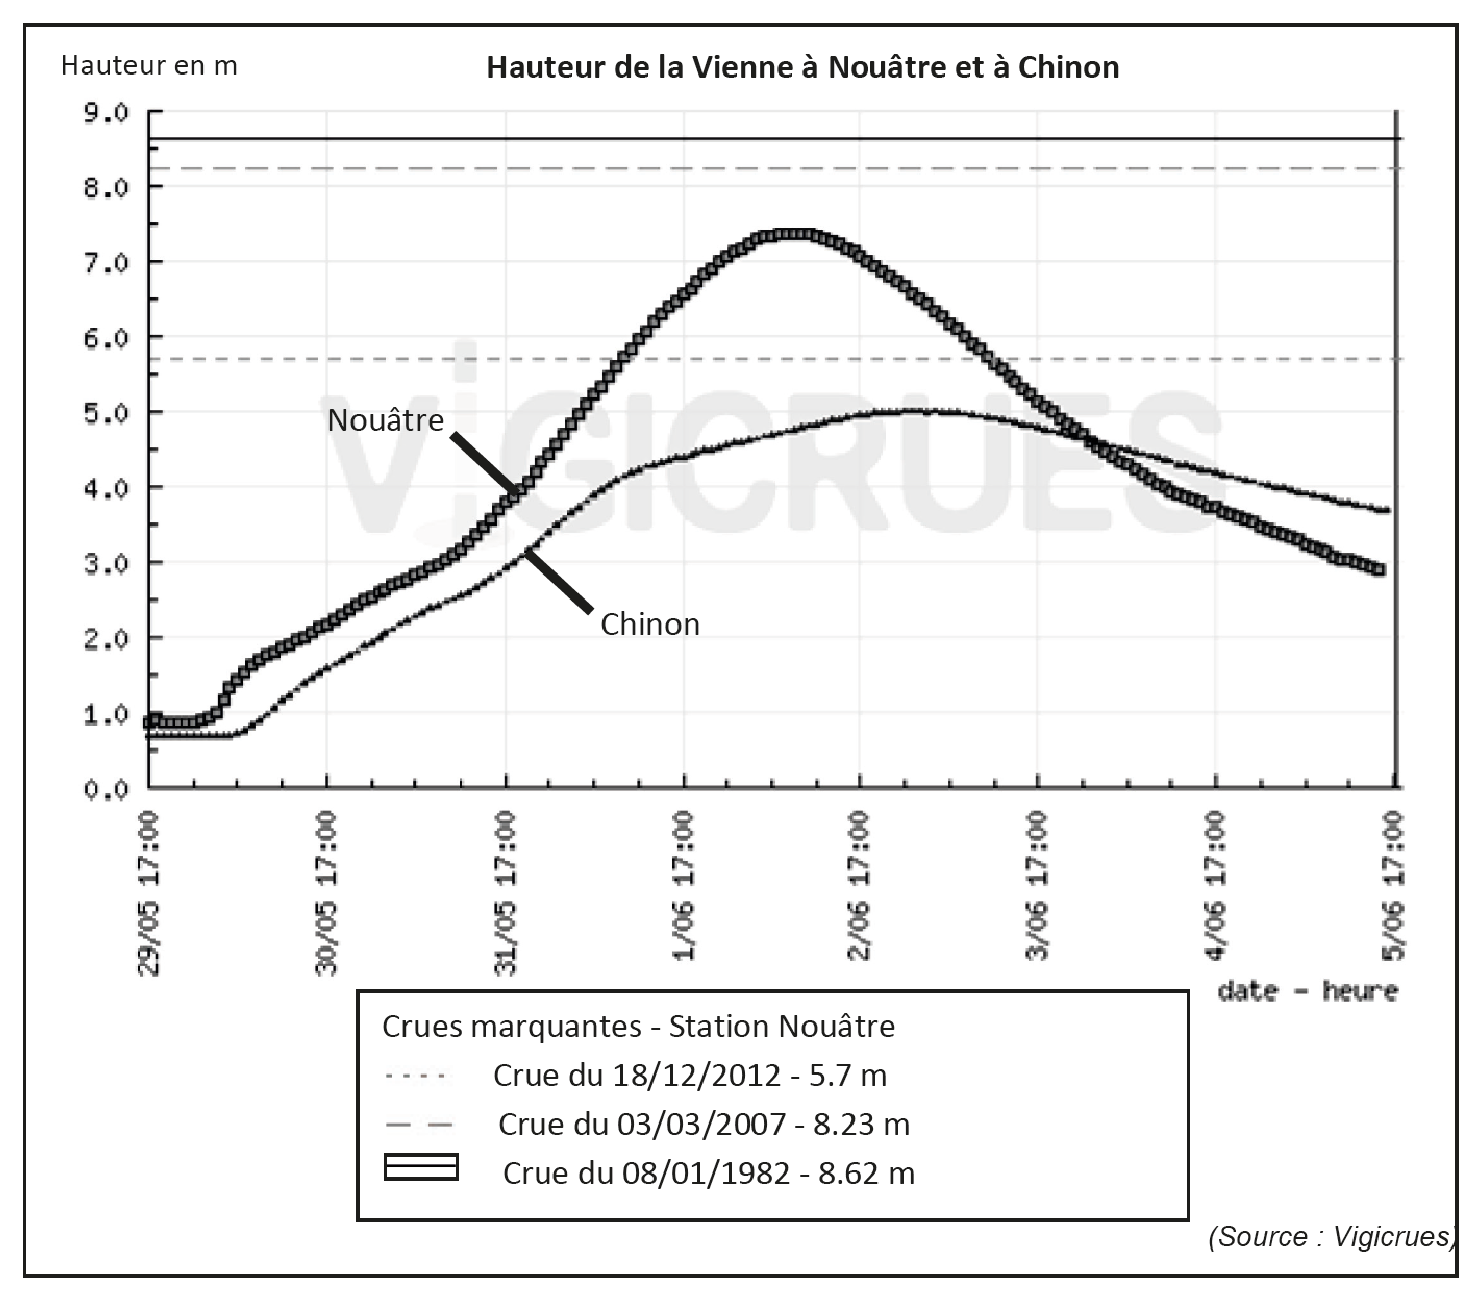
\includegraphics[width=12cm]{Organisation_gestion_donnees/Images/D5_ex_vigicrues}
%\end{center}
%À l’aide du graphique ci-dessus, répondre aux questions suivantes.
%\begin{enumerate}
%   \item Quelle hauteur maximale la Vienne a-t-elle atteinte à Chinon entre le 29 mai 2016 à 17h et le 5 juin 2016 à 17h ?
%   \item À Nouâtre, entre le 29 mai 2016 à 17h et le 5 juin 2016 à 17h, pendant combien de temps le niveau de l’eau a-t-il été supérieur au niveau maximum de la crue du 18 décembre 2012 ? Donner la réponse en heure.
%   \item
%   \begin{enumerate}
%      \item Combien d’heures se sont écoulées entre le pic de la crue de Nouâtre et celui de Chinon ?
%      \item De Nouâtre ou de Chinon, quelle station est située le plus en amont de la rivière ? Justifier la réponse.
%   \end{enumerate}
%\end{enumerate}
%\end{exercice*}
%
%\begin{corrige}
%\ \\ [-5mm]
%\begin{enumerate}
%   \item Entre le 29 mai 2016 à 17h et le 5 juin 2016 à 17h, la hauteur maximale à Chinon a été d'environ {\blue 5 mètres}.
%   \item Entre le 29 mai 2016 à 17h et le 5 juin 2016 à 17h, le niveau de l’eau à Nouâtre a été supérieur au niveau maximum de la crue du 18 décembre 2012 pendant environ {\blue 50 heures}.
%   \item
%   \begin{enumerate}
%      \item Environ {\blue 18 heures} se sont écoulées entre le pic de la crue de Nouâtre et celui de Chinon.
%      \item {\blue Nouâtre} est la station située le plus en amont de la rivière puisqu'elle possède le pic de crue en premier.
%   \end{enumerate}
%\end{enumerate}
%\end{corrige}


%\begin{exercice*}[CRPE 2014 G3] %%%%%%%%%%%%
%   Optimisation du volume d'un moule. \\
%   On fabrique un moule de pâtisserie (sans couvercle) dans une plaque de métal carrée de côté 10 cm en découpant un petit carré dans chaque coin puis en pliant comme suit :
%   \begin{center}
%      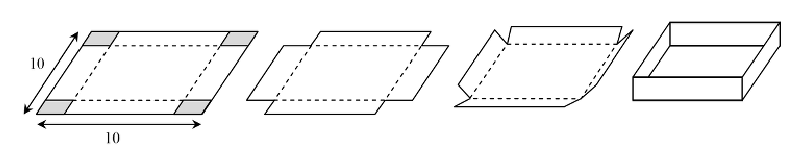
\includegraphics[width=13cm]{Organisation_gestion_donnees/Images/D5_ex_moule}
%   \end{center}  
%   \vspace*{-0.8cm}
%   \begin{enumerate}
%      \item Parmi les quatre graphiques ci-dessous, quel est celui qui représente le volume du moule (en cm\up{3}) obtenu en fonction de la longueur des côtés des carrés découpés (en cm) ? Justifier.
%      \begin{center}
%      \begin{tabular}{cC{1}c}
%         {\psset{xunit=0.5,yunit=0.05}
%          \begin{pspicture}(0,-10)(12,115)
%             \multido{\i=1+1}{11}{\psline[linecolor=gray](\i,0)(\i,105)}
%             \multido{\i=10+10}{10}{\psline[linecolor=gray](0,\i)(11.5,\i)}  
%             \psaxes[Dx=1,Dy=10,labelFontSize=\scriptstyle]{->}(0,0)(11.5,105)
%             \psplot[algebraic=true,linewidth=1.5pt]{0}{10}{-4*(x-5)^2+100}  
%         \end{pspicture}}
%         & &
%         {\psset{xunit=1,yunit=0.05}
%          \begin{pspicture}(0,-10)(6,115)
%             \multido{\n=0.5+0.5}{11}{\psline[linecolor=gray](\n,0)(\n,105)}
%             \multido{\i=10+10}{10}{\psline[linecolor=gray](0,\i)(5.5,\i)}  
%             \psaxes[Dy=10,labelFontSize=\scriptstyle]{->}(0,0)(5.5,105)
%             \psplot[algebraic=true,linewidth=1.5pt]{0}{5}{x*(10-2*x)^2}  
%         \end{pspicture}} \\
%         {\it graphique 1} & & {\it graphique 2} \\
%         {\psset{xunit=1,yunit=0.07}
%          \begin{pspicture}(0,-7)(6,85)
%             \multido{\n=0.5+0.5}{10}{\psline[linecolor=gray](\n,0)(\n,80)}
%             \multido{\i=5+5}{15}{\psline[linecolor=gray](0,\i)(5.5,\i)}  
%             \psaxes[dx=0.5,Dy=10,dy=5,labelFontSize=\scriptstyle]{->}(0,0)(5.5,80)
%             \psplot[algebraic=true,linewidth=1.5pt]{0}{5}{x*(10-2*x)^2} 
%         \end{pspicture}} 
%         & &    
%         {\psset{xunit=0.5,yunit=0.05}
%          \begin{pspicture}(0,-10)(12,110)
%             \multido{\i=1+1}{11}{\psline[linecolor=gray](\i,0)(\i,105)}
%             \multido{\i=10+10}{10}{\psline[linecolor=gray](0,\i)(11.5,\i)}  
%             \psaxes[Dx=1,dx=2,Dy=10,dy=20,labelFontSize=\scriptstyle]{->}(0,0)(11.5,105)
%             \psplot[algebraic=true,linewidth=1.5pt]{0}{10}{-4*(x-5)^2+100}  
%         \end{pspicture}} \\
%         {\it graphique 3} & & {\it graphique 4} \\
%      \end{tabular}
%      \bigskip
%      \end{center}   
%      \item Par lecture graphique, encadrer par deux entiers consécutifs la longueur du côté qui permet d'obtenir le volume maximal.
%   \end{enumerate}  
%\end{exercice*}
%
%\begin{corrige}
%\ \\ [-5mm]
%\begin{enumerate}
%   \item Pour un petit carré de côté 1 cm par exemple, le volume du moule en cm$^3$ sera de $8\times8\times1 =64$. \\
%   Donc, il s'agit du {\blue graphique 2}.
%   \item On lit {\blue $1<\ell<2$.}
%\end{enumerate}
%\end{corrige}


